\documentclass[11pt,a4paper]{article}
\pdfoutput=1

\usepackage[utf8]{inputenc}
\usepackage{amsmath}
\usepackage{amsfonts}
\usepackage{textcomp}
\usepackage{graphicx}
\usepackage{authblk}
\usepackage{subfig}
\usepackage{gensymb}

% COMMENT THIS LINE FOR ARXIV SUBMISSION
\graphicspath{{figs/}}

\begin{document}

\title{Space CoBot: a collaborative aerial robot for indoor microgravity
  environments}
\author{Pedro Roque}
\author{Rodrigo Ventura}
\affil{%
  Institute for Systems and Robotics \\
  Instituto Superior Técnico, Universidade de Lisboa \\
  Av. Rovisco Pais, 1; 1049-001 Lisboa, Portugal \\
  {\small pedro.roque@tecnico.ulisboa.pt} \\
  {\small rodrigo.ventura@isr.tecnico.ulisboa.pt}}
\date{}
\maketitle

\begin{abstract}
  This paper presents a first contribution to the design of a small
  aerial robot for inhabited microgravity environments, such as
  orbiting space stations. In particular, we target a fleet of robots
  for collaborative tasks with humans, such as telepresence and
  cooperative mobile manipulation. We explore a propeller based
  propulsion system, arranged in such a way that the translational and
  the rotational components can be decoupled, resulting in an holonomic
  hexarotor. Since propellers have limited thrust, we employ an
  optimization approach to select the geometric configuration
  given a criteria of uniform maximum thrust across all directions in
  the body reference frame. We also tackle the problem of motion
  control: due to the decoupling of translational and rotational modes
  we use separate converging controllers for each one of these
  modes. In addition, we present preliminary simulation results in a
  realistic simulator, in closed loop with the proposed controller,
  thus providing a first validation of the followed methodology.
\end{abstract}

\section{Introduction}
\label{sec:introduction}

Multirotor vehicles have recently gained widespread use in various
application areas, such as transportation, surveillance, and even
entertainment. These platforms are mechanically simple and typically
lightweight, resulting in a low cost of acquisition and
maintenance. However, to the best knowledge of the authors, there is
no known application of multirotor vehicles in space
environments. Discarding the obvious impossibility of maneuvering in
the absence of air, we consider here the use of these vehicles in
human-compatible pressurised spaces under microgravity, such as inside
inhabited space stations.

The idea of aerial vehicles inside space stations is not new. The NASA
project SPHERES (Synchronized Position Hold Engage Reorient
Experimental Satellites) started in 2000 with the design of a small
pressurised air propulsion vehicle~\cite{miller00}. In 2006 three
SPHERES units were deployed aboard the International Space Station
(ISS)~\cite{nolet07}.  However, the use of pressurised air makes the
mechanical complexity significantly higher than a multirotor based
solution.  More recently, NASA proposed the Astrobee vehicle, with a
simpler propulsion system based on several centrifugal fans and
nozzles~\cite{bualat15}. The Astrobee also features a 2 DoF arm and
docking capability.

The most prominent feature of these spaces is the absence of gravity
exerted in bodies, that is, the gravity force canceled
by the orbital motion of the air mass (microgravity). We will exploit this feature in
the following way. Most multirotor orient their propellers
vertically along parallel axes. This maximizes thrust vertically in
order to compensate for the gravity force. However, in doing so they
need to tilt in order to move sideways. Moreover, most of the energy
is spent in compensating for gravity. In its absence, not
only there is no need to compensate for gravity, but also the
energy consumption is expected to be significantly less. We propose
to orient the propeller rotation axes non-parallel among them, in
such a way we obtain a fully actuated body. That is, to be able
to decouple translational from rotational motion. We expect to
increase maneuverability, being a particularly relevant feature inside
confined spaces such as the interior of a space station.

Fully actuated multirotor have been proposed in the past, but the
literature is scarce. In~\cite{jiang13,voyles12} a dexterous
hexarotor has been proposed, where the fully actuation feature is
used for dexterous manipulation. However, this vehicle is designed for
Earth applications, and thus a tradeoff is necessary between dexterity
and gravity compensation. Our design is also based in an hexarotor,
but since we consider microgravity, we will design the propeller
orientation in order to maximize maneuverability along all directions.

The goal of this paper is to present a design of an hexarotor for
microgravity environments. We target a multipurpose vehicle, and
provide as working examples (1)~telepresence, requiring the vehicle to
manoeuvre in such a way the screen and camera is pointer towards the
party onboard, and (2)~mobile manipulation, requiring force closure in
order to compensate the reaction force at the end effector. We also
consider operational issues such as docking into a charging station
and stacking of multiple units in order to save space.

This paper is structured as follows: the requirements and
specifications we considered, including a preliminary mechanical
design for the vehicle are explained in
Section~\ref{sec:vehicle-design}, in Section~\ref{sec:dynamical-model} we
derive a parametric dynamical model of the vehicle, which is then used
in Section~\ref{sec:design-parameters} for the optimization of the
propellers orientation. Section~\ref{sec:posit-attit-contr} proposes a
convergent controller for this fully actuated vehicle, and a
preliminary validation in a realistic simulation environment is
presented in Section~\ref{sec:prel-valid}, while
Section~\ref{sec:concl-future-work} wraps up the paper with concluding
remarks and a reference for future work.


%%% Local Variables: 
%%% mode: latex
%%% TeX-master: "main"
%%% End: 


\section{Vehicle design}
\label{sec:vehicle-design}
%UNUSED: \input{vd.tex}

\subsection{Requirements}
\label{sec:requirements}
% The Space CoBot is an approach to a microgravity UAV, capable of omnidirectional flying, to operate inside the International Space Station, as well as other microgravity atmosphered environments. In the development process, we selected the following guidelines: 

As starting point for the design of the aerial vehicle we considered
the following requirements:
\begin{enumerate}
\itemsep=0em
\item Safe operation;
\item Self-contained and simple propulsion system, with holonomic
  kinematics, that is, capable of motion in an arbitrary direction;
\item Autonomous Guidance, Navigation and Control (GN\&C);
\item Small dimensions;
\item Modularity;
\item Stackability and docking.
\end{enumerate}
An holonomic kinematics implies the decoupling between translational
and rotational motion. That is, the vehicle should not be required to
change attitude to move in a given direction. This requirement,
together with the one of small dimensions is particularly relevant
inside confined spaces such are those of space stations. We also
require the vehicle to have an autonomous GN\&C, thus simplifying the
deployment in already equipment-dense space environments. Modularity is
relevant to not only simplify maintenance, but also to allow the vehicle
to be extensible. Stackability and docking targets not only the dock
into a charging station, but also the possibility of parking them one
 on top of the others, thus saving space.

%%% Local Variables:
%%% mode: latex
%%% TeX-master: "main"
%%% End:


\subsection{Specification}
\label{sec:specification}

Our proposed solution is based on an multirotor vehicle, where the propellers are placed in such a way that full holonomy is attained. That is, fully decoupling the translational from the rotational motion, resulting in a 6 Degrees-of-Freedom (DoF) vehicle. The minimum amount of propellers is thus~6, since each propeller corresponds to a single DoF. We propose electric propulsion, due to its simplicity. Since there is no need to compensate for gravity, we expect the energy consumption to be significantly lower than conventional multirotors on Earth.

On Figure~\ref{fig:overall} we provide a preliminar render for the proposed solution.
\begin{figure}
  \centering
  \subfloat[]{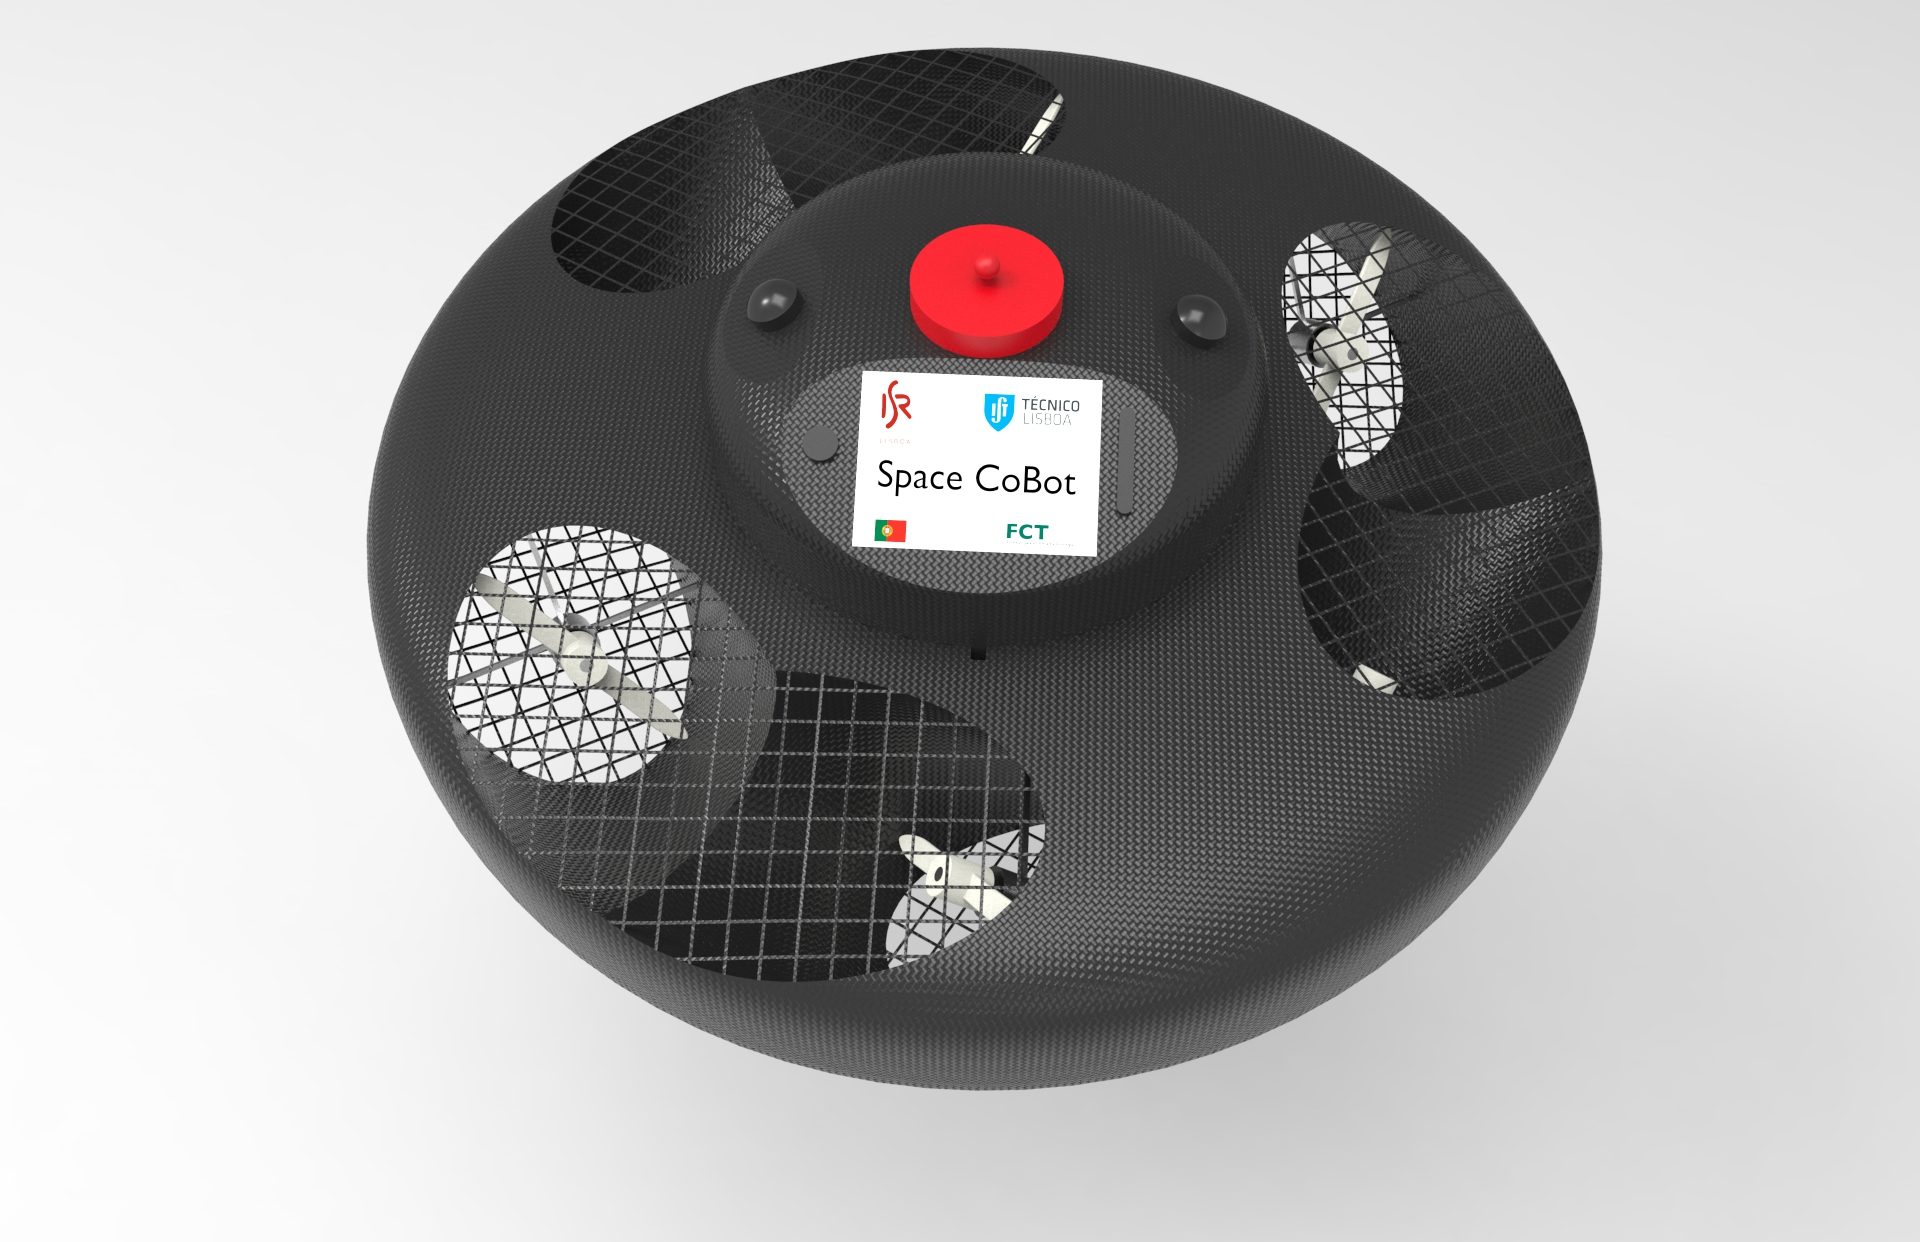
\includegraphics[height=0.33\linewidth]{provided_sol.jpg}} \hfill
  \subfloat[]{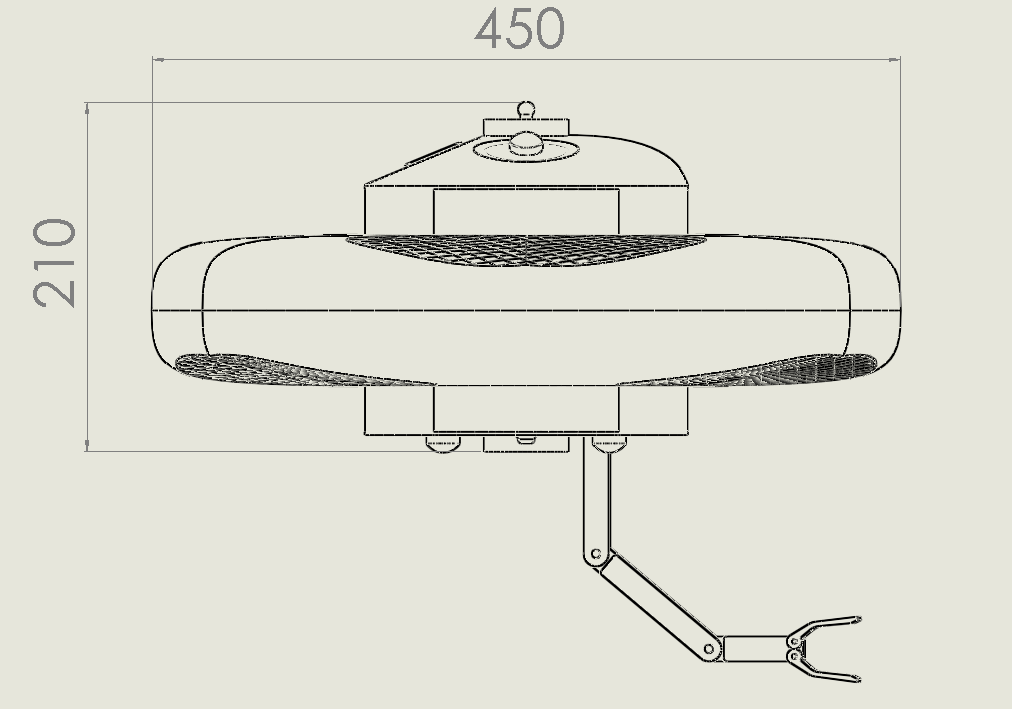
\includegraphics[height=0.33\linewidth]{Side_View_Tech.png}}
  \caption{Render of the overall view of Space CoBot (left) and its external dimensions (right).}
  \label{fig:overall}
\end{figure}
It is based on 6 electrically powered propellers, protected inside the
hull of the vehicle. On the top of the vehicle one can find the
docking port, two wide-angle cameras for telepresence and vision-based
navigation, and a screen (with the size of a common smartphone). At the bottom one can find another docking port for stacking, and two more wide-angle cameras. In the following subsections we explain how our design addresses each one of the above mentioned requirements.

The size of the robot in our design is 450mm by 210mm, with a maximum free volume of 2.4 liters for guest modules and experiments. Several images of the Space CoBot are presented below, as well as the overall dimensions in Figure~\ref{fig:overall}(b).

\subsubsection{Safety}

Safety is a priority on any object, manned or unmanned, aboard a space station. This poses a problem, as most robots are source of acoustic and electromagnetic noise, which shall be kept at a minimum. Along this, we also have the problem of moving objects, such as the propellers, which may cause debris shall any foreign object hit them.

In order to cope with electromagnetic noise, each section of the robot
is covered with grounded copper mesh that actuates as a Faraday
cage. All motors are protected with a carbon grid to prevent floating
objects of reaching the propellers while they are spinning. Proximity
sensors are also disposed around the propellers airflow tunnel, to
detect and stop the motor in case a small object reaches the propulsion system. To make the vehicle as silent as possible, acoustic absorbing material is placed around the motors cavity. 

% ???This also prevents the robot of operating inside the station for larger periods of time, as this is a limiting factor.


\subsubsection{Propulsion System}

Taking advantage of the pressurized atmosphere inside a space station, the proposed propulsion system employs six motors, each with a 4 inches propeller.  
The selection of electric motors for the propulsion system aims at safety, as it does not have to deal with highly pressurized gas tanks, and can be used with interchangeable batteries or fast-charge docking systems. All the 6 motors are placed along the same plane, 60 degrees away from each other. Each motor is, then, tilted 55 degrees from its vertical axis, providing holonomic motion and enabling total force closure. We defer the justification for this angle to Section~\ref{sec:design-parameters}.
All propellers are kept inside the propulsion module and airflow is driven through net protected vents, so to avoid foreign objects of reaching the propeller. The suggested propulsion system is shown in Figure~\ref{fig:propulsion_system}.

\begin{figure}
  \centering
  \subfloat[]{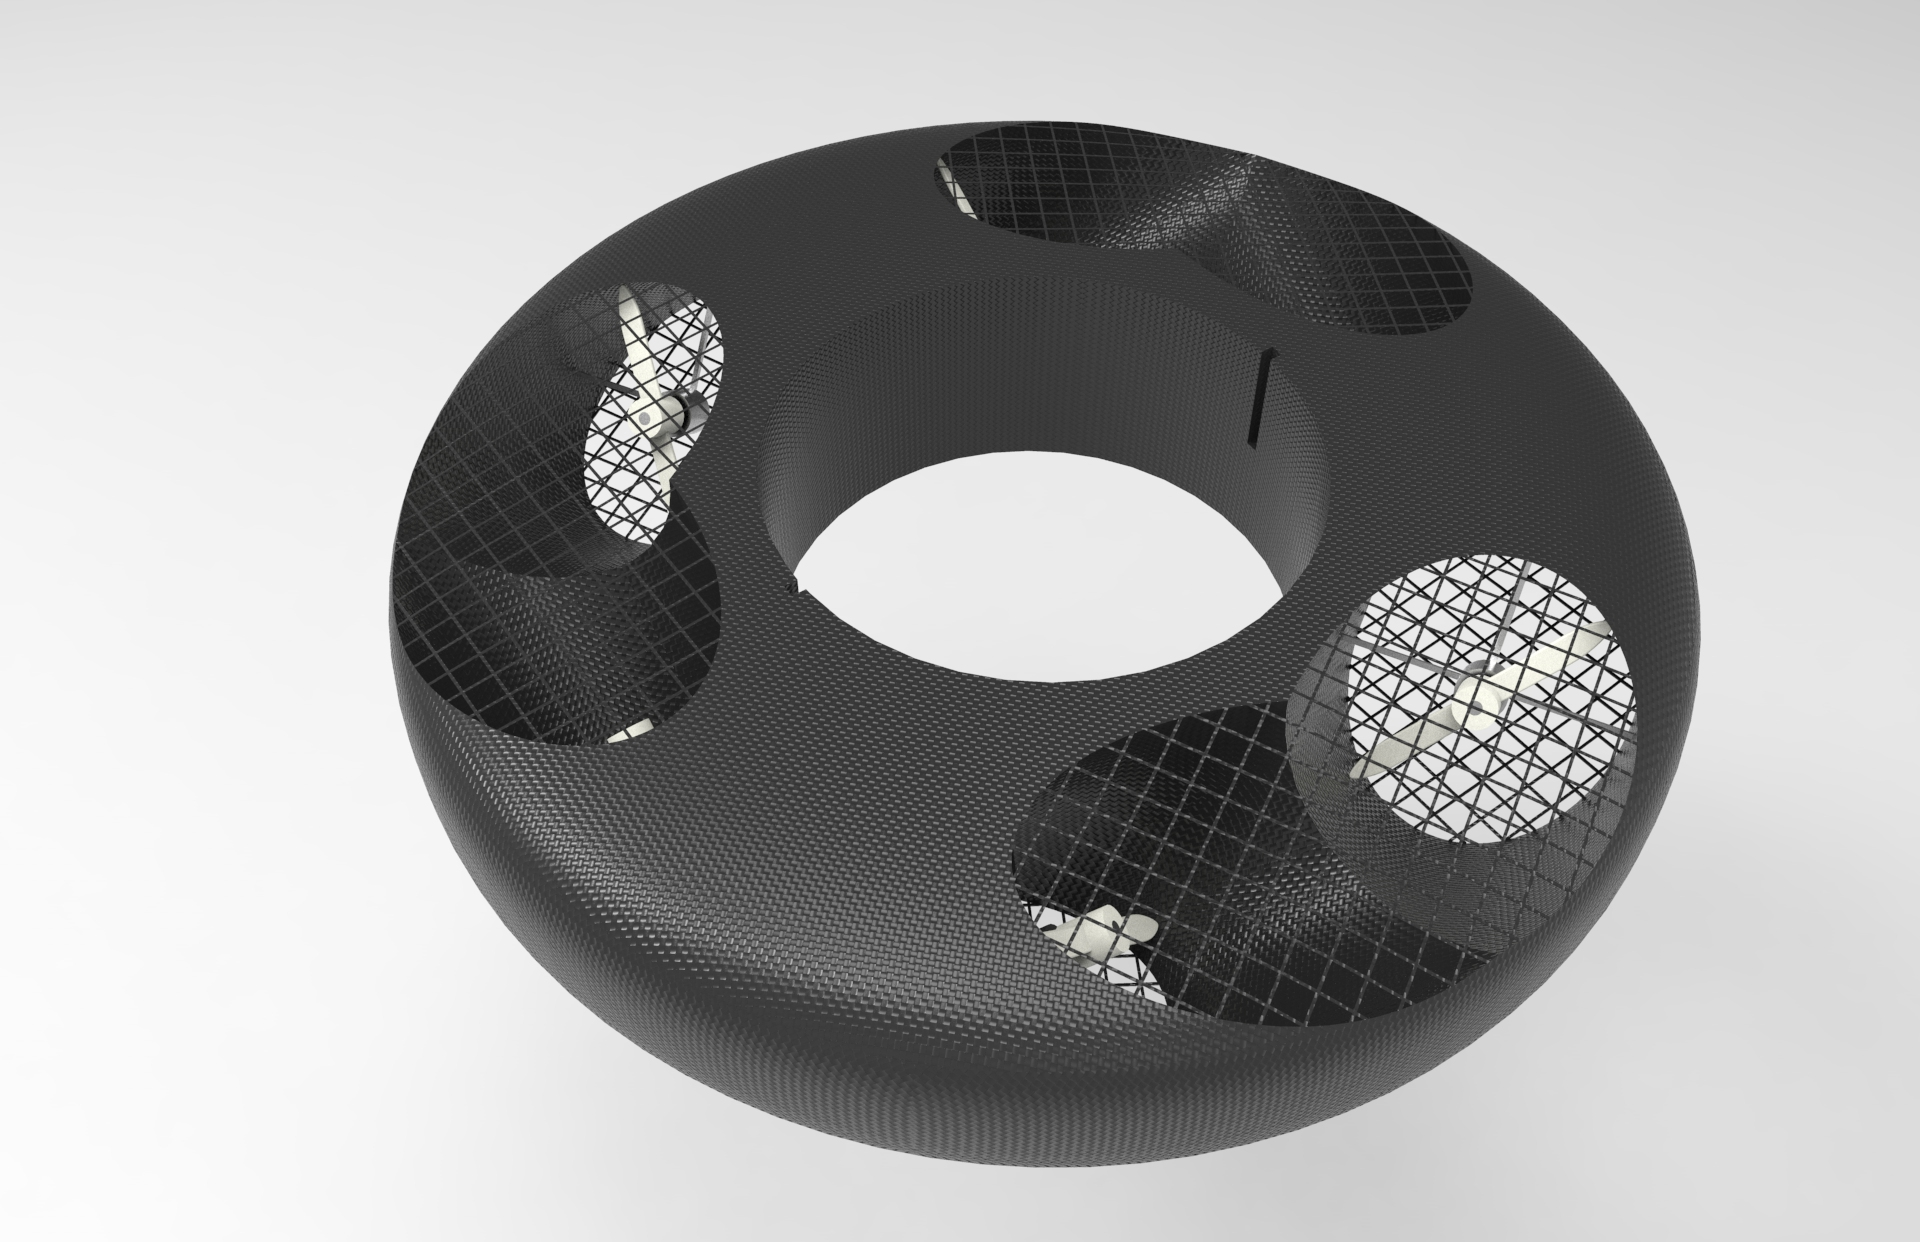
\includegraphics[width=0.49\linewidth]{propulsion_shell.jpg}} \hfill
  \subfloat[]{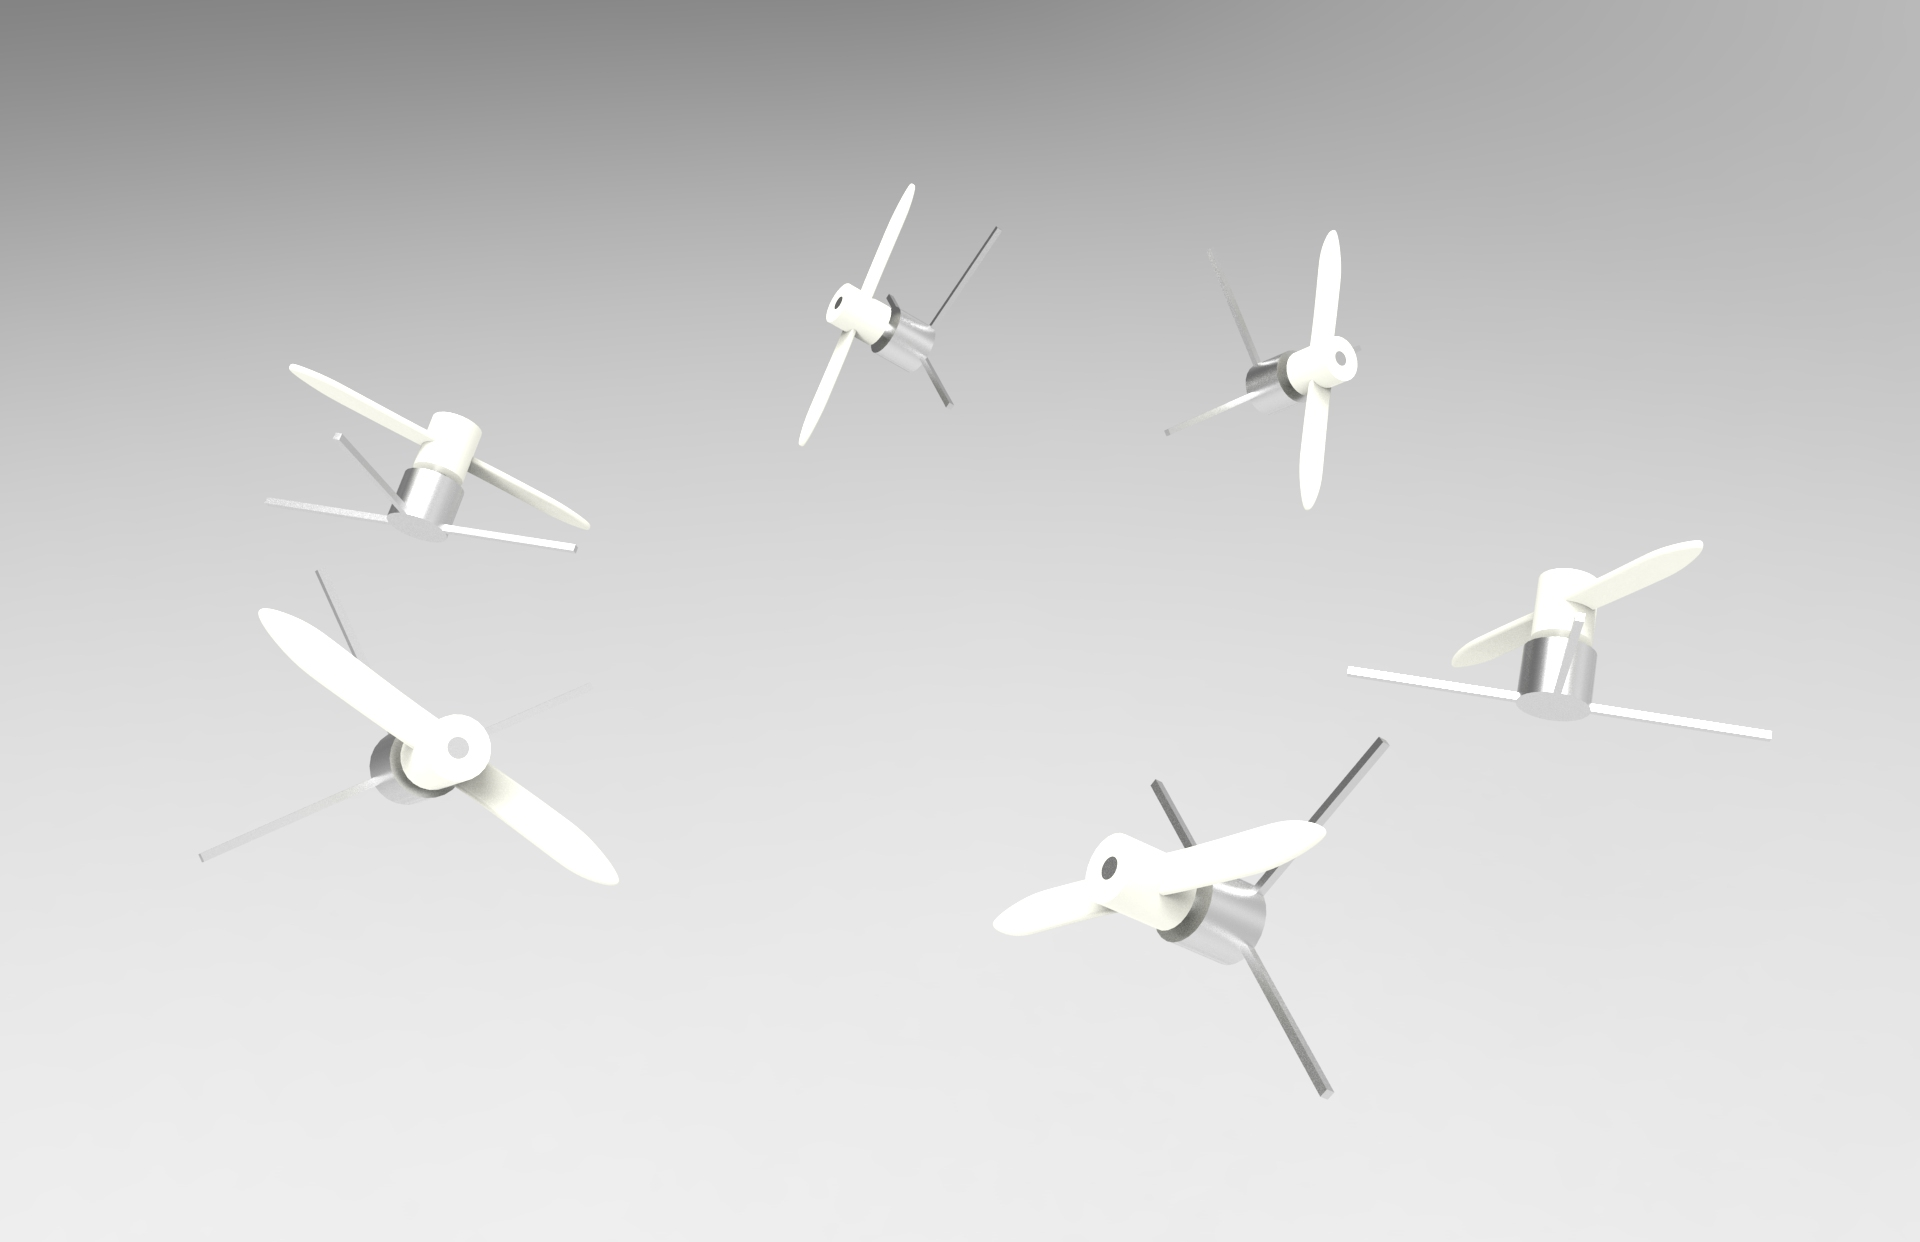
\includegraphics[width=0.49\linewidth]{propulsion_system.jpg}}
  \caption{Propulsion system representation: (a)~overall view of the module, and (b)~relative placement of the propellers.}
  \label{fig:propulsion_system}
\end{figure}


\subsubsection{GN\&C System}

The navigation and guidance system is based on four wide-angle cameras spread on the top and bottom parts of the device, providing total coverage around the robot. To obtain reliable position and orientation inside the Space Station, robust vision-based algorithms are used in order to locate and navigate the robot. For instance, a combination of stereo and monocular features may be used as proposed in~\cite{yoda:ssrr12fj}.

The control system is composed of a hardware layer and a software stack. 
The hardware layer is composed by a core system, supporting the base navigation functionalities, and guest systems, allowing for extension modules and scientific payloads. They interface through a distributed communication layer based on parallel protocols. Figure~\ref{fig:comm_module} represents the architecture. In green we represent low-level communications and on red high-level ones.

\begin{figure}
  \centering
  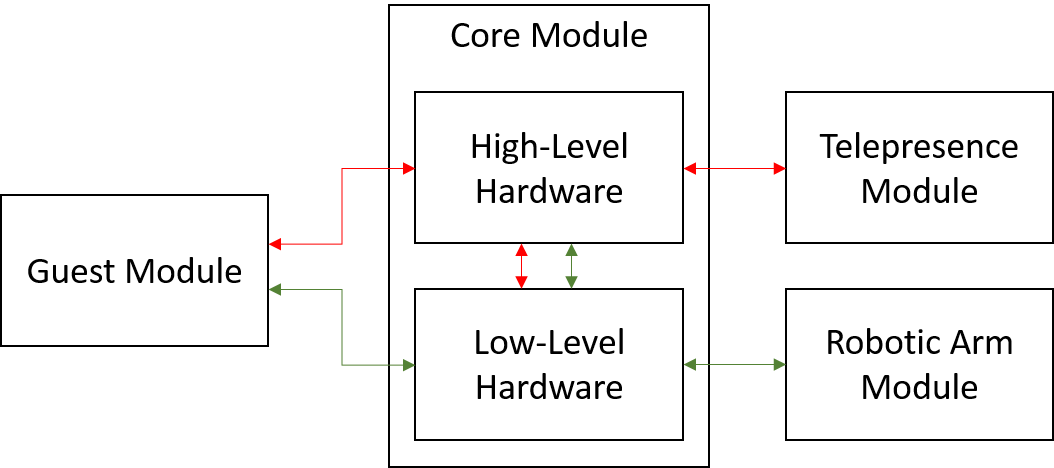
\includegraphics[width=0.7\linewidth]{com_network.png}
  \caption{Communications between the various modules of the vehicle.}
  \label{fig:comm_module}
\end{figure}

On the software side, a low-level autopilot is responsible for basic
pose stabilization and motor driving system, relying on the low-level
hardware layer. High-performance algorithms can be deployed on the
high-level hardware layer, such as vision-based localization and
telepresence audio and video streaming.

%is capable of trajectory planning and mission scheduling, as well as remote operation (either through Ground Control Station or by any astronaut).

\subsubsection{Modularity}

A crucial requirement for maintenance procedures is modularity. For this purpose, we divided the Space CoBot into several detachable modules:
\begin{enumerate}
	\item \emph{Backbone module}: the backbone module provides support for all modules and constitutes the main component of the Space CoBot. It has slots for all modules, provides data connection through all subsystems and it is capable of delivering power to all components. It provides mounting points for 4~wide-angle cameras for navigation, two on the bottom part of the robot and two on the top side. Also, contains a dome module with a telepresence kit (small computer with a screen, webcam, microphone, and speaker), as well as two wide-angle cameras. Modules are attached through a drawer system, with mechanic and magnetic locking, enabling easy swap-on and preparation for all experiments. Two types of drawers can be used: one with 550 cubic centimeters (standard drawer), and other with 1200 cubic centimeters (double height drawer, approximately). 
	\item \emph{Propulsion module}: contains all the 6 motors, propellers, and Electronic Speed Controllers (ESC). Connects to the backbone module through low level communication protocols, such as CAN (to provide control on each motor), and two power cables.
	\item \emph{Core module}: contains core GN\&C systems. It can be fitted into a standard or double height drawer, depending on the computational modules or volume for experiments. A Space CoBot can have simultaneously multiple high-level Core modules (for increased computational power), but only one low-level core module.
	\item \emph{Guest modules}: provides the possibility of extending CoBot's functionality with additional modules, such as experimental test-beds for microgravity;
	\item \emph{Robotic arm module}: a robotic arm with 4 DoF is provided, allowing manipulation of objects (such as operational knobs) or grasping dock bars. This module fits in a standard drawer and must be replaced on the bottom slot of the vehicle. If no robotic arm is needed, one may replace the drawer with an additional guest module.
\end{enumerate}

Each module is easily accessible due to the robot layout, and thus it can be easily replaced. A view of all the modules is available on Figure~\ref{fig:explosion}.

\begin{figure}
  \centering
  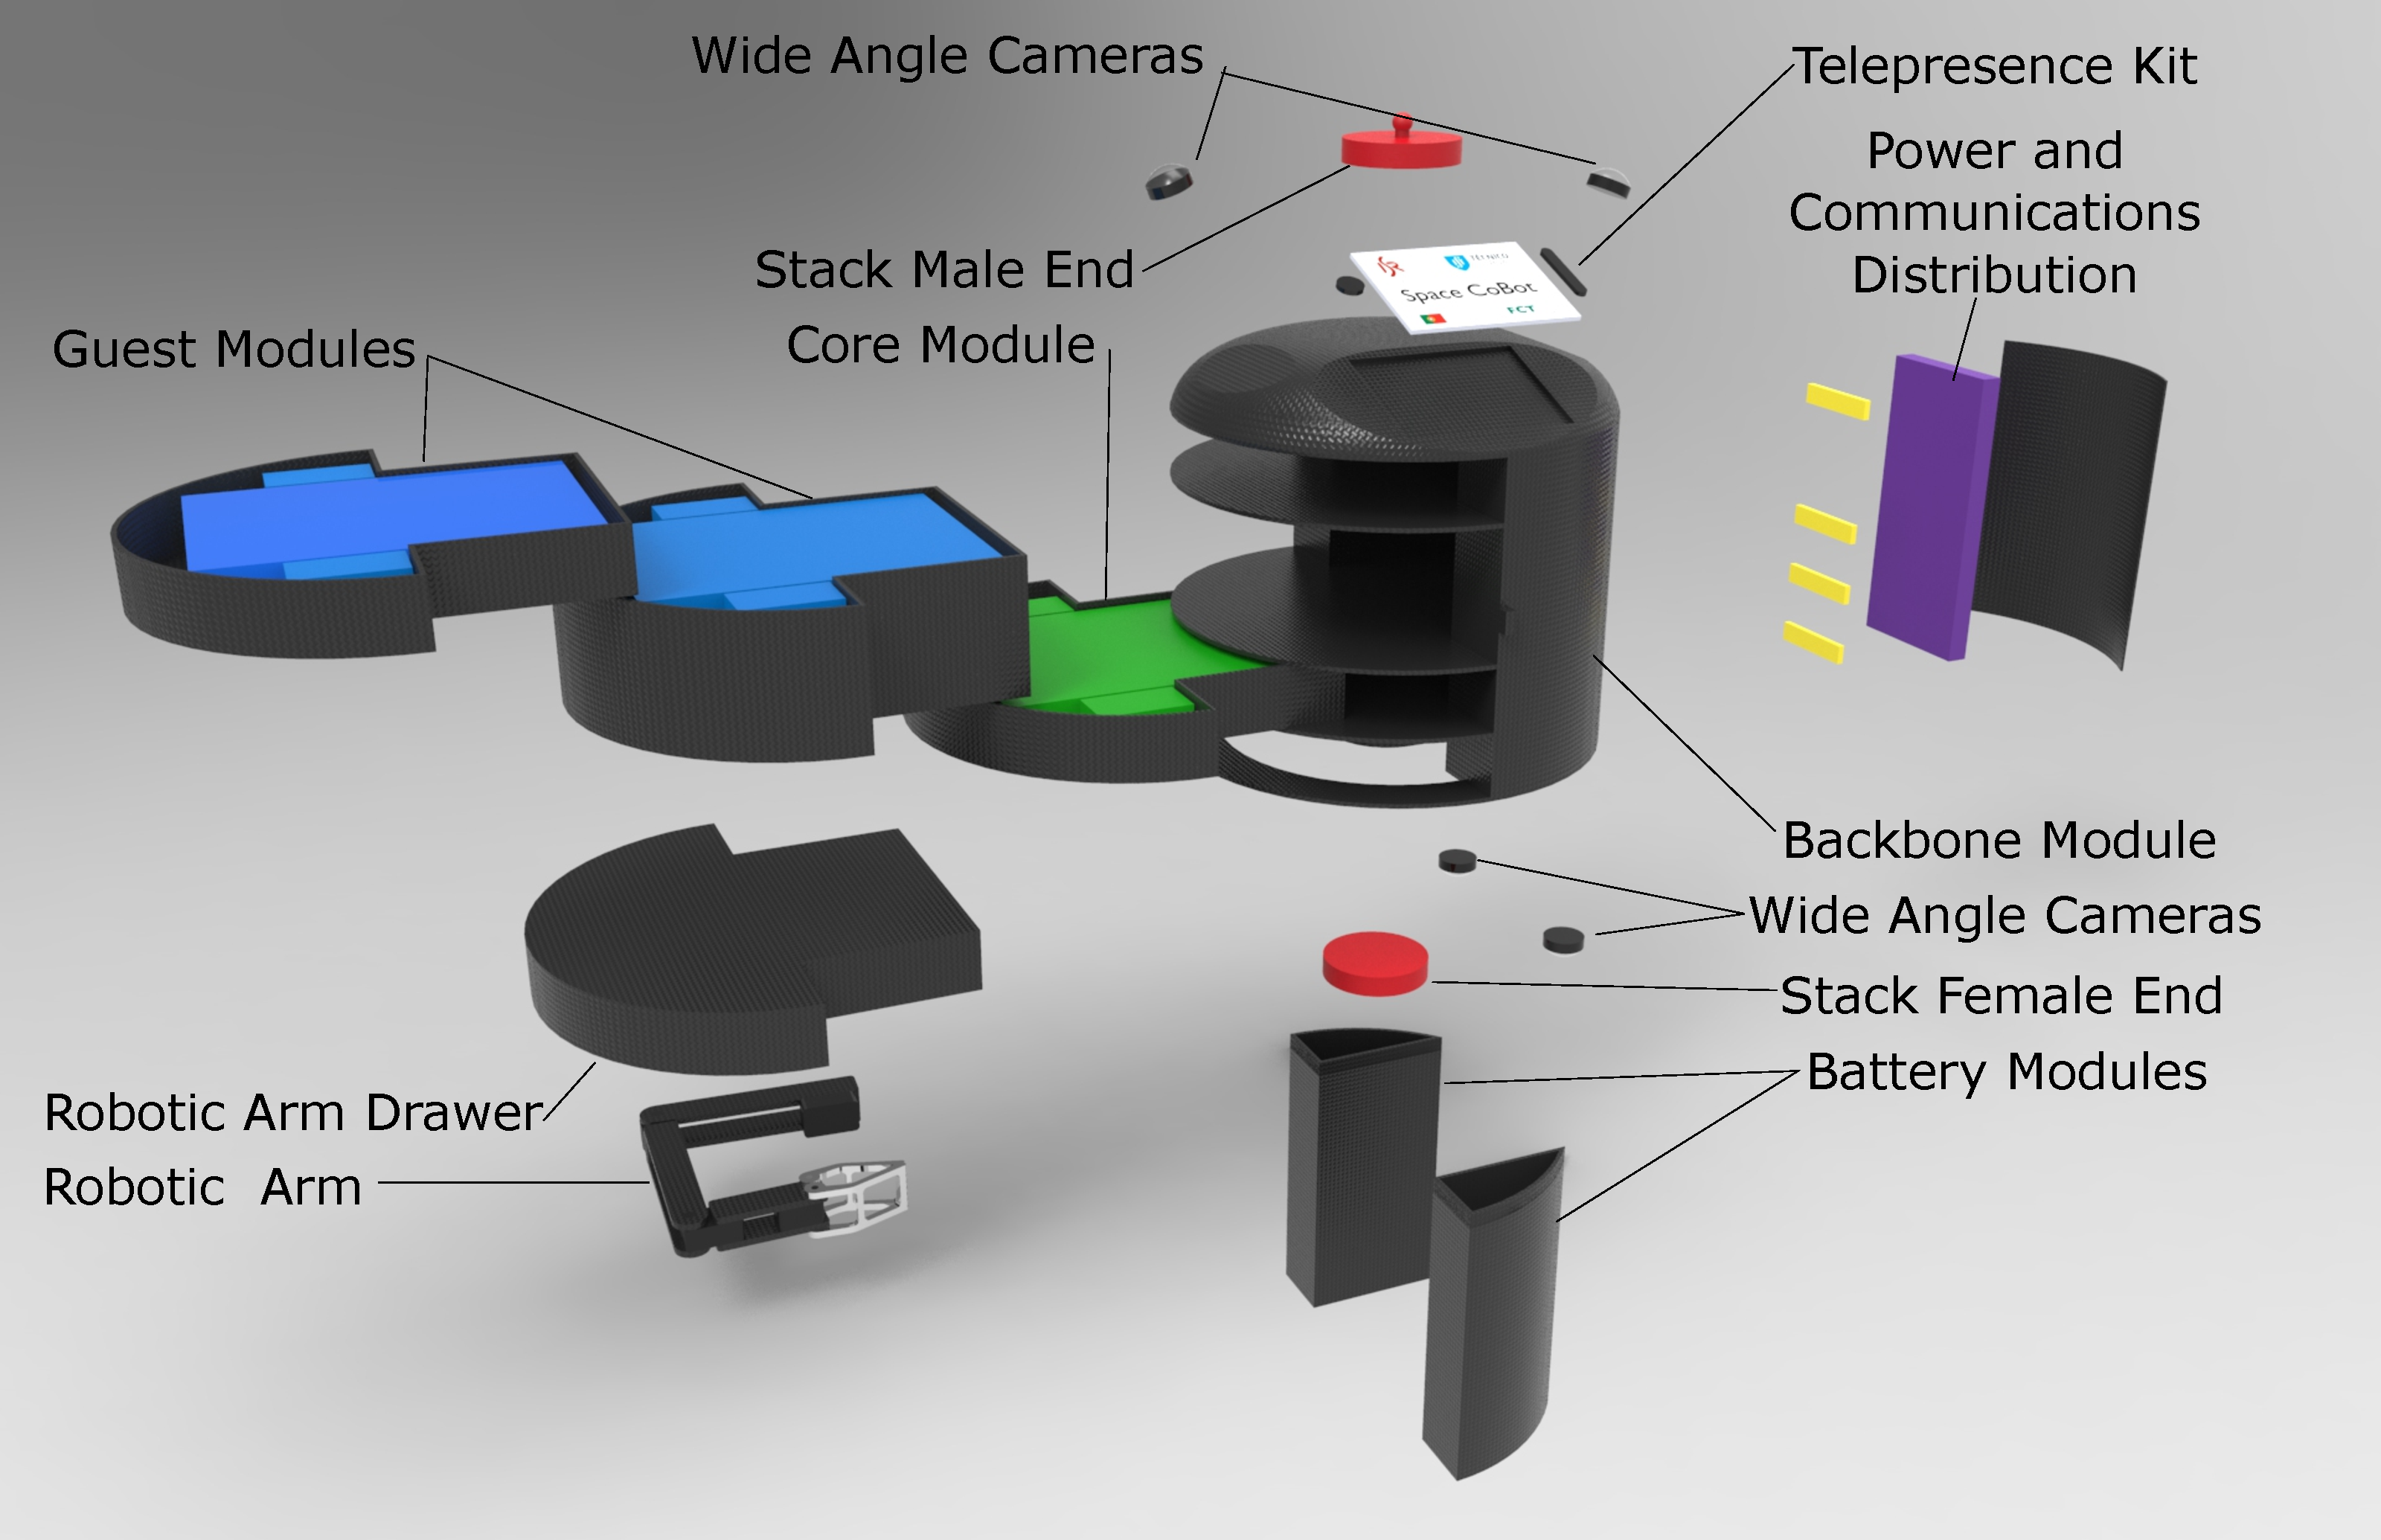
\includegraphics[width=0.9\linewidth]{new-explosion.pdf}
  \caption{Vehicle modules, excluding propulsion module (see Figure~\ref{fig:propulsion_system}).}
  \label{fig:explosion}
\end{figure}

\subsubsection{Stackability}

Stackability ensures compact storage of the Space CoBots when charging. All Space CoBots have two stacking components: a male port, at the top, and a female end, at the bottom. These components are placed on opposite sides of the robot, providing physical and electrical coupling. Its cylindrical symmetry simplify docking, as the heading of the robot is not relevant for a successful connection. When stacked, a power connection is made and we are able to charge several Space CoBots at the same time. When one Space CoBot is fully charged, it can detach itself from the stack and the remain robots may re-attach themselves. Figure~\ref{fig:coupled} shows two coupled robots and a detail view of the coupling mechanism. This mechanism is loosely based on the one proposed in~\cite{yoda:raposa:industrial} for a land robot.

\begin{figure}
  \centering
  \subfloat[]{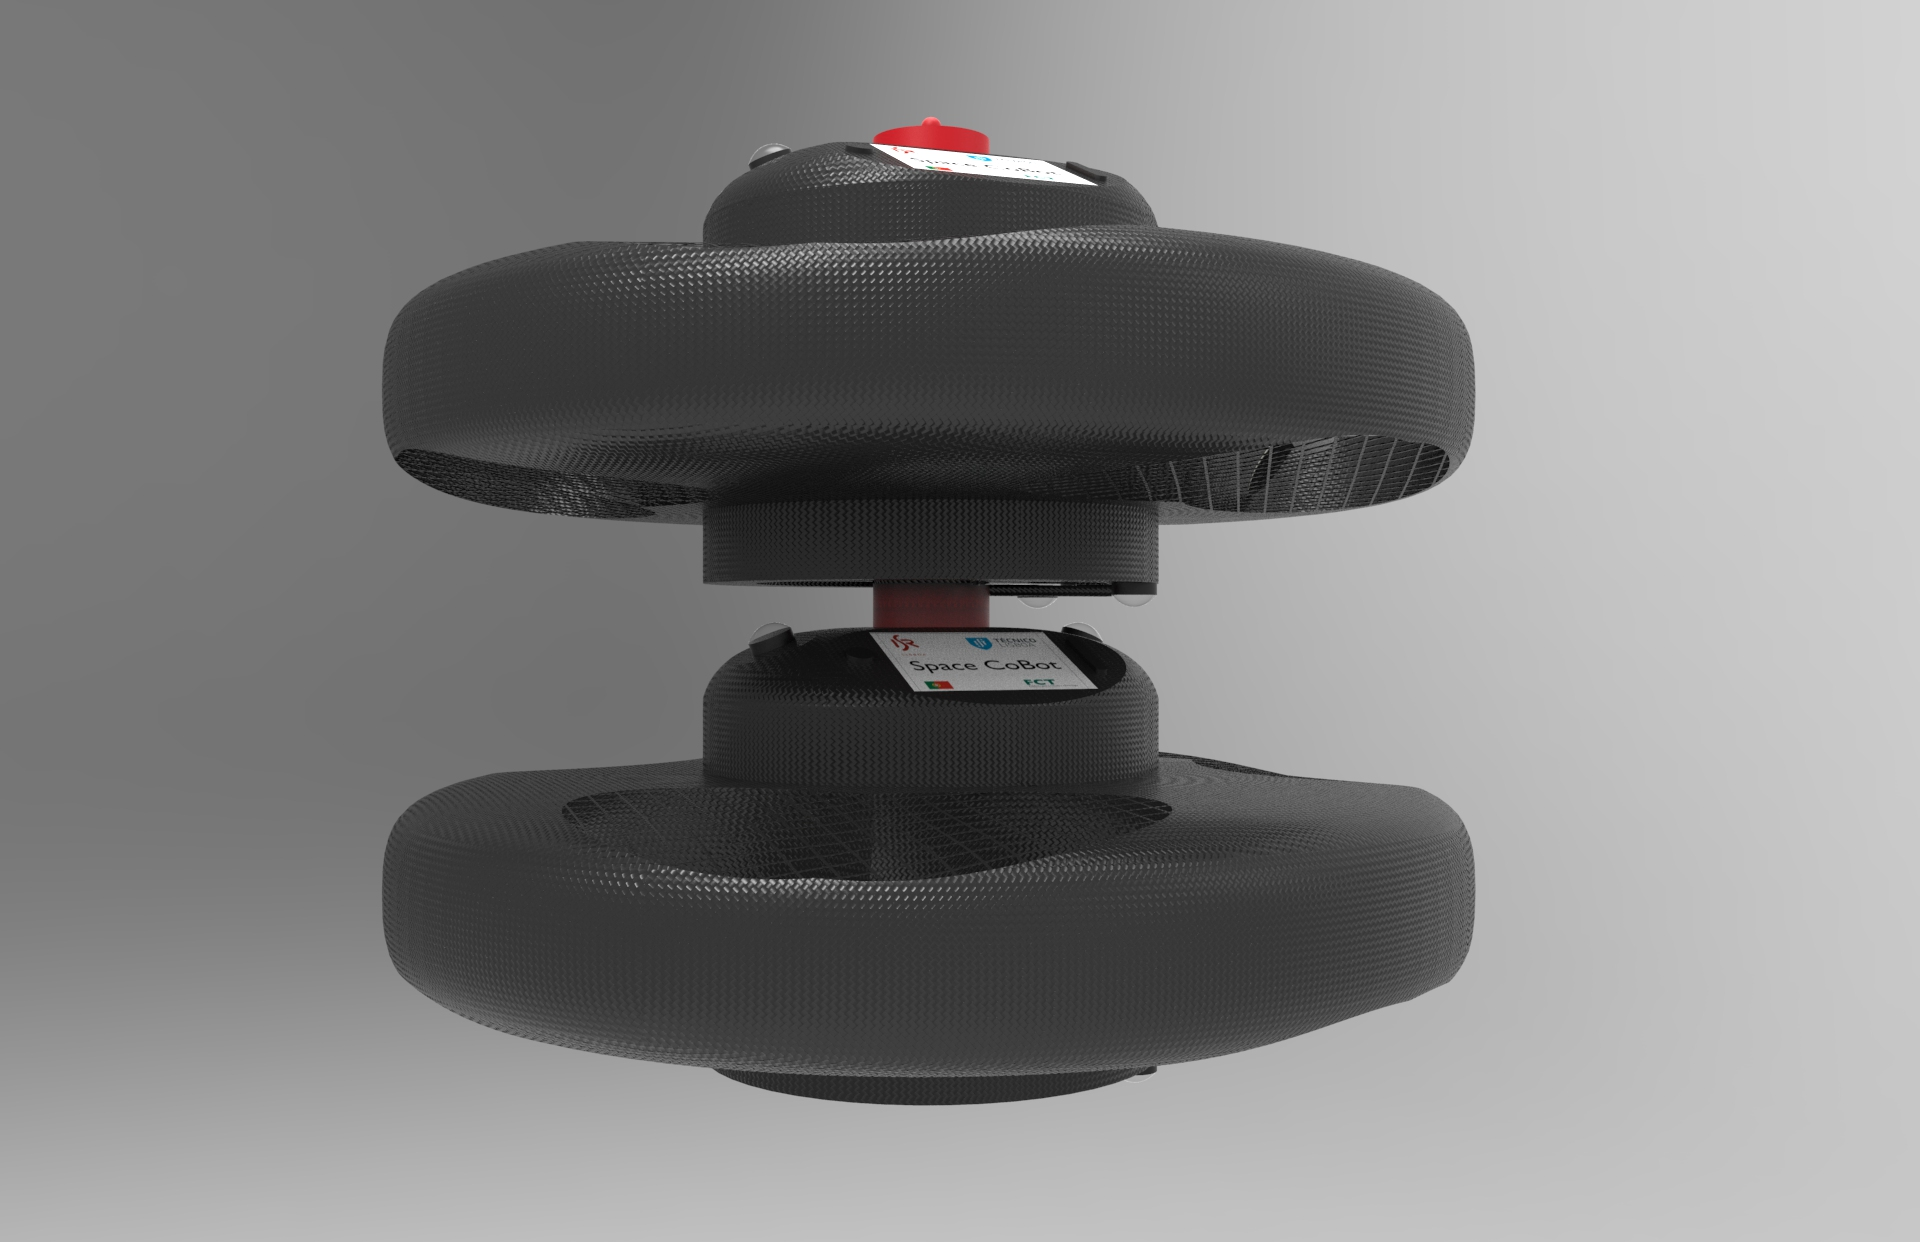
\includegraphics[width=0.49\linewidth]{coupling-view.jpg}} \hfill
  \subfloat[]{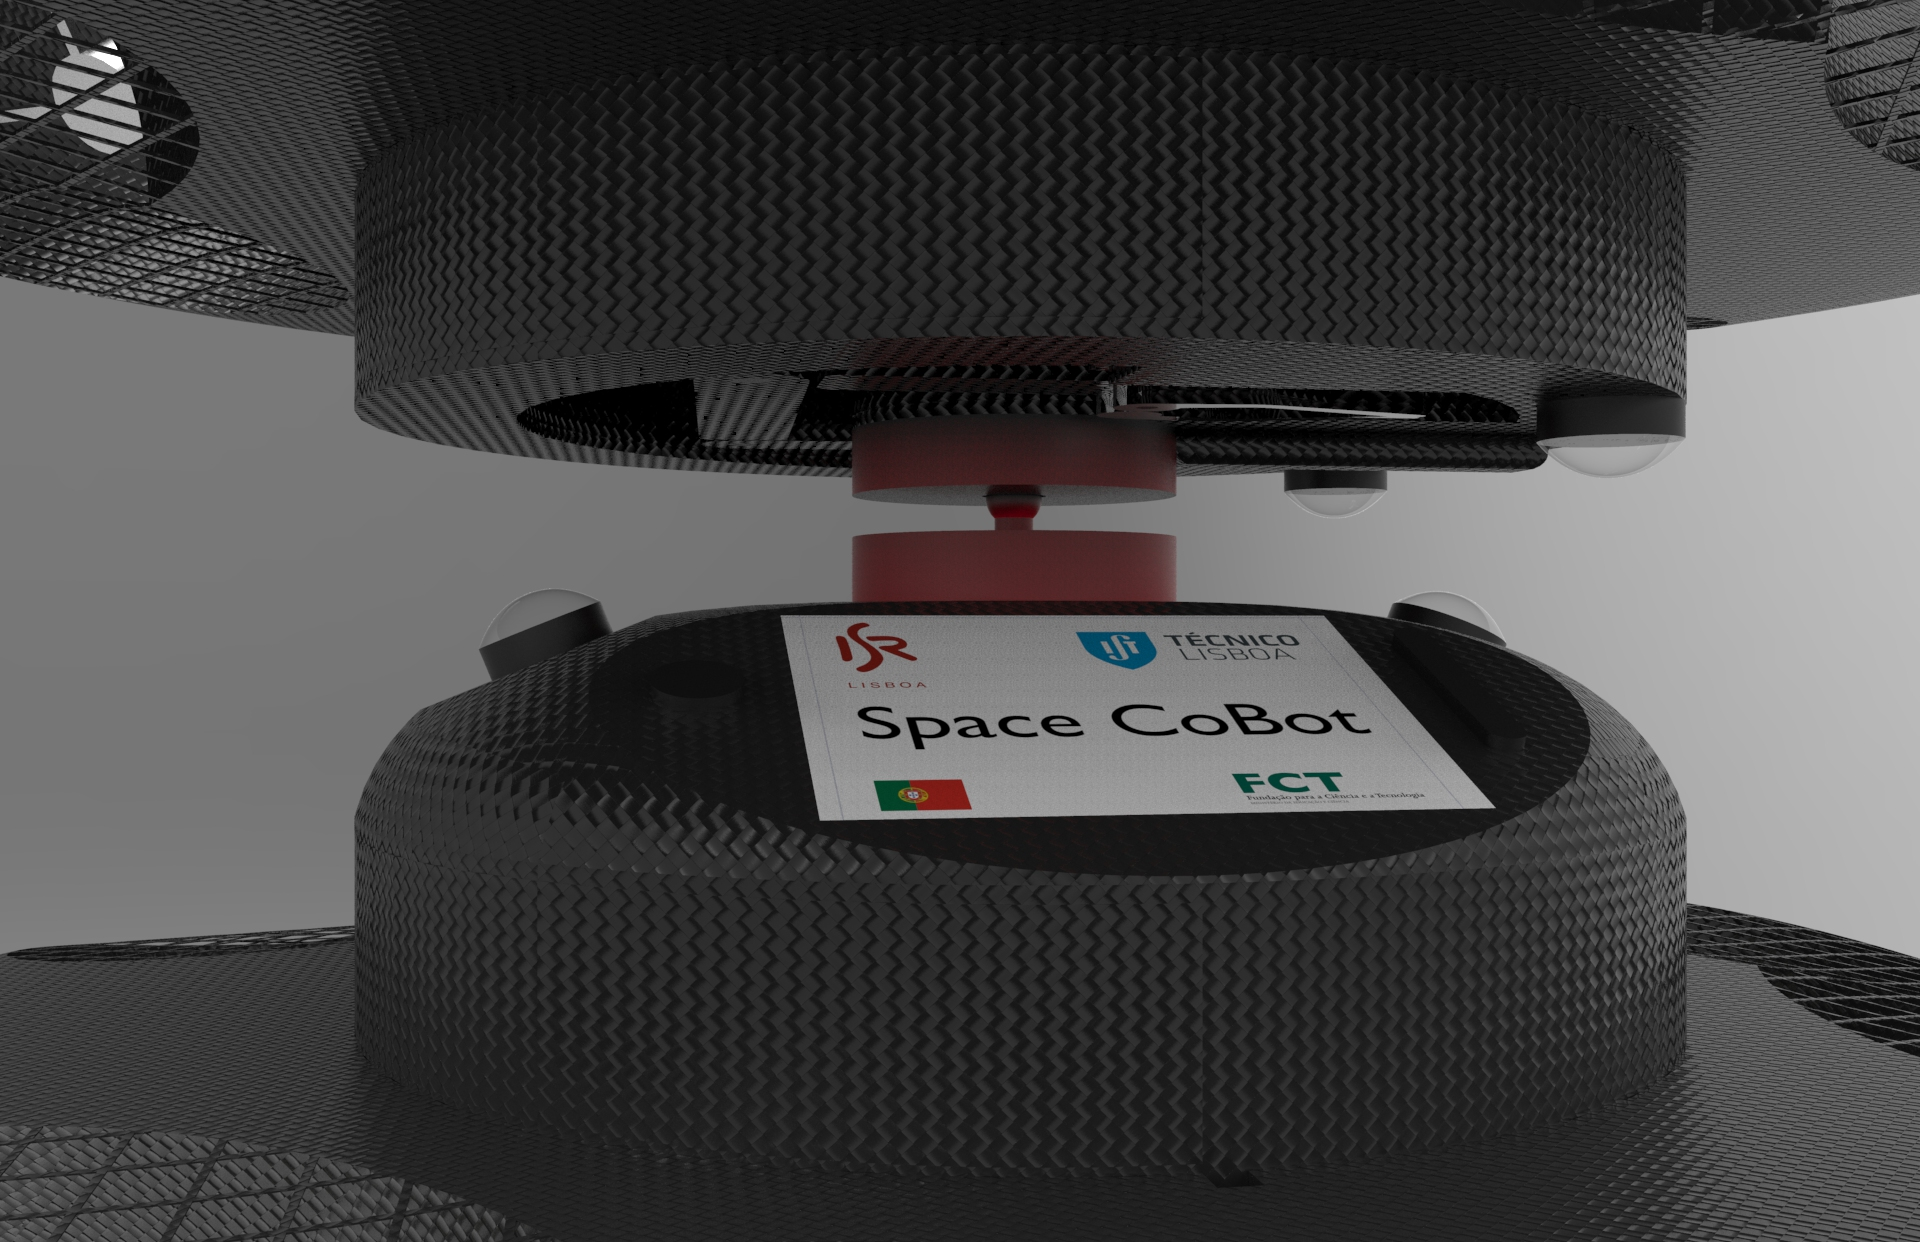
\includegraphics[width=0.49\linewidth]{coupling-detail.jpg}}
  \caption{Left: two Space CoBots coupled together; right: coupling mechanism detail.}
  \label{fig:coupled}
\end{figure}

%%% Local Variables:
%%% mode: latex
%%% TeX-master: "main"
%%% End:


\section{Dynamical model}
\label{sec:dynamical-model}

To derive the dynamical model of the vehicle, we start by modeling the
force and torque vectors caused by a single propeller in the body
frame denoted~$\mathcal{B}$, whose origin is coincident with the
vehicle's center of mass (CoM).

Consider a propeller $i$ whose motor is rigidly linked to the
body frame, as depicted in Figure~\ref{fig:prop}.  This propeller will
generate a force $\bar{F}_i$ and a torque $\bar{M}_i$ with respect to
the CoM. While the former results directly from the
propeller thrust,
\begin{align}
  \label{eq:Fi}
  \bar{F}_i &= f_i \hat{u}_i \\
  f_i &= K_1 u_i
\end{align}
where $u_i$ is the actuation signal and $f_i$ is the scalar thrust,
the later has two components: the torque caused by the displaced force
and the propeller reaction torque:
\begin{align}
  \label{eq:Mi}
  \bar{M}_i &= \bar{r}_i\times\bar{F}_i - \tau_i \hat{u}_i \\
  \tau_i &= w_i K_2 u_i
\end{align}
where $\times$ denotes vector cross product and $w_i$ is $-1$ or $1$ depending on whether the propeller rotates
clockwise or anti-clockwise for a positive forward thrust $f_i>0$.
The constants $K_1$ and $K_2$ model a simple linear relationship
between the actuation and the scalar thrust force and reaction torque
of the propeller. The actuation is often modeled as proportional to
the square of the propeller speed of rotation~\cite{mahony12}.

The relative position of the propeller, $\bar{r}_i$, orthogonal to the
$Z$ axis, and the unit vector $\hat{u}_i$, aligned with the propeller
axis, are uniquely defined by the angles $\theta_i$ and $\phi_i$, and can be
easily obtained from geometrical reasoning:
\begin{equation}
  \bar{r}_i = \left(
    \begin{array}{c}
      d\cos(\theta_i) \\
      d\sin(\theta_i) \\
      0
      \end{array}
    \right)
    \qquad
    \hat{u}_i = \left(
      \begin{array}{c}
        \sin(\theta_i)\sin(\phi_i) \\
        -\cos(\theta_i)\sin(\phi_i) \\
        \cos(\phi_i)
      \end{array}
      \right)
\end{equation}
where $d=\|\bar{r}_i\|$ is the distance from the propeller to the CoM.
Stacking together the resulting force $\bar{F}_i$ and torque
$\bar{M}_i$, one can obtain the linear relation
\begin{equation}
  \label{eq:fm}
  \left(
    \begin{array}{c}
      \bar{F}_i \\
      \bar{M}_i
    \end{array}
  \right) = \bar{a}_i\,u_i
\end{equation}
where
\begin{equation}
  \begin{split}
    \bar{a}_i  &= \left(
      \begin{array}{c}
        K_1 \hat{u}_i \\
        K_1 \bar{r}_i \times \hat{u}_i - w_i K_2 \hat{u}_i
      \end{array}
    \right) \\
    &= \left(
      \begin{array}{c}
        K_1 \sin(\theta_i)\sin(\phi_i) \\
        -K_1 \cos(\theta_i)\sin(\phi_i) \\
        K_1 \cos(\phi_i) \\
        (K_1 d \cos(\phi_i) - w_i K_2 \sin(\phi_i))\sin(\theta_i) \\
        -(K_1 d \cos(\phi_i) - w_i K_2 \sin(\phi_i))\cos(\theta_i) \\
        -K_1 d \sin(\phi_i) - w_i K_2 \cos(\phi_i)
      \end{array}
    \right)
    \end{split}
\end{equation}

\begin{figure}
  \centering
  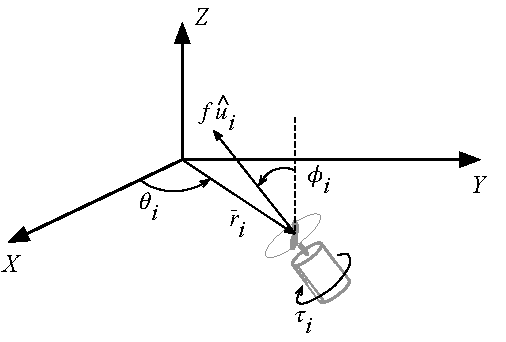
\includegraphics[width=0.6\linewidth]{prop.pdf}
  \caption{Notation used for modeling a single propeller with respect
    to the body frame~$\mathcal{B}$, centered on the vehicle's CoM.}
  \label{fig:prop}
\end{figure}

For a vehicle with $N$ propellers, the resulting force and torque will
be given by the sum of the contributions of each propeller, given with
respect to the CoM, by~\eqref{eq:fm}. This sum can be put in matrix
form as
\begin{equation}
  \label{eq:au}
  \left(
    \begin{array}{c}
      \bar{F} \\
      \bar{M}
    \end{array}
  \right) = \mathbf{A}\,\bar{u}
\end{equation}
where $\mathbf{A}=[\bar{a}_1 \cdots \bar{a}_N]$, hereby called
\emph{actuation matrix}, and $\bar{u}=[u_1\cdots u_N]^T$, the
actuation input vector. The crucial observation is that, if the
actuation matrix $\mathbf{A}$ has at least rank 6, the six degrees of
freedom of the force and torque combined can be decoupled by
solving~\eqref{eq:au} with respect to the actuation~$\bar{u}$. A
necessary (but not sufficient) condition for this to be true is to have at least 6
propellers, as in the hexarotor design considered in this paper. Note
that this matrix only depends on the vehicle's design parameters,
defined by the angles $\{\theta_i\}$ and $\{\phi_i\}$, distance $d$,
and the trust coefficients $K_1$, $K_2$, and $\{w_i\}$. However, we
will defer the discussion about the properties of this matrix to the
next section.

The dynamical model of the vehicle, in the absence of gravity can be
derived from the Newton and Euler equations of motion, similarly
to~\cite{mahony12}. Let us denote the position and velocity of the
body frame $\mathcal{B}$ with respect to the inertial frame
$\mathcal{I}$ as $\bar{x}$ and $\bar{v}$, the rotation matrix of frame
$\mathcal{B}$ with respect to $\mathcal{I}$ as $\mathbf{R}$, and the
angular velocity of the vehicle in the body frame $\mathcal{B}$ as
$\bar{\omega}$. Then,
\begin{equation}
  \label{eq:dynsys}
  \left\{
    \begin{aligned}
      \dot{\bar{x}} &= \bar{v} \\
      m \dot{\bar{v}} &= \mathbf{R} \bar{F} \\
      \dot{\mathbf{R}} &= \mathbf{R}\,\mathbf{S}(\bar{\omega}) \\
      \mathbf{J} \dot{\bar{\omega}} &= \bar{M} - \bar{\omega}\times\mathbf{J} \bar{\omega}
    \end{aligned}
  \right.
\end{equation}
where the constants $m$ and $\mathbf{J}$
are the vehicle's mass and moment of inertia, while
$\mathbf{S}(\bar{\omega})$ is the skew-symmetric matrix defined by
\begin{equation}
  \label{eq:S}
  \mathbf{S}(\bar{\omega}) =
  \left[
    \begin{array}{ccc}
      0 & -\omega_z & \omega_y \\
      \omega_z & 0 & -\omega_x \\
      -\omega_y & \omega_x & 0 \\
    \end{array}
  \right]
\end{equation}
for $\bar{\omega}=[\omega_x\:\omega_y\:\omega_z]^T$.

%%% Local Variables:
%%% mode: latex
%%% TeX-master: "main"
%%% End:


\section{Optimization of the design parameters}
\label{sec:design-parameters}

In this section we will study how the design parameters translate into
the actuation matrix $\mathbf{A}$ defined in the previous section. In
particular, we will consider how a bounded actuation translates into
maximum values of force and torque. We will then optimize these
parameters in order to maximize these values across all directions.

\subsection{Problem statement}
\label{sec:problem-statement}

% Throughout this paper we will assume that the propellers are equally
% distributed radially, that is,
% \begin{equation}
%   \label{eq:thetas}
%   \theta_i = (i-1) \frac{\pi}{3}
% \end{equation}
% For the sake of symmetry we will further consider the rotation
% directions to be alternating, that is,
% \begin{equation}
%   \label{eq:ws}
%   w_i =
%   \begin{cases}
%     1 & i\text{ is odd,} \\
%     -1 & i\text{ is even.}
%   \end{cases}
% \end{equation}

We will start by considering that each actuation signal is
bounded between $-1$ and $1$, that is,
\begin{equation}
  \label{eq:ahcube}
  -1 \leq u_i \leq 1 \quad \text{for} \quad i=1,\ldots,6
\end{equation}
According to \eqref{eq:au}, this hypercube will map onto a
6-dimensional convex polyhedron\footnote{A convex polyhedron is an
  intersection of a finite number of half-spaces~\cite{jeter86}.} in
the $(\bar{F}, \bar{M})$ space.  Any other choice of bounds is
possible by appropriately scaling constants $K_1$ and $K_2$.  However,
it assumes that the maximum propeller trust is symmetric with respect
to the direction of rotation. The remaining parameters are the angles
$\{\phi_i\}$. We will base our analysis on the optimization of these
angles with respect to various criteria.

Our goal will be to find the configurations of angles $\{\phi_i\}$
that maximize the range of forces (and torques) over all
directions. Conventional multirotors have all propellers directed at
the same direction, \textit{i.e.,} with $\{\phi_i=0\}$,, which
maximizes the thrust along that direction. However, they are unable to
produce any thrust component over an orthogonal direction. By having
nonzero values of $\{\phi_i\}$
we expect to gain thrust over any direction, at the
expense of reducing the maximum thrust over some particular one.
Geometrically, this corresponds to changing $\{\phi_i\}$
such that a ball of nonzero radius can fit inside the 3-dimensional
convex polyhedron in the $\bar{F}$ space mapped by the actuation
hypercube in~\eqref{eq:ahcube}, while keeping zero torque,
$\bar{M}=0$. A similar reasoning applies to the torque space
$\bar{M}$, while keeping $\bar{F}=0$. In sum, we will look for the values of $\{\phi_i\}$ that
maximize these radii.

First, we will address the problem of computing the maximum force
along a given direction specified as a unit vector $\hat{e}$, while
maintaining a zero torque.  From~\eqref{eq:au}, and assuming that
$\mathbf{A}$ is full rank, we get
\begin{equation}
  \bar{u} = \mathbf{A}^{-1}
  \left(
    \begin{array}{c}
      \bar{F} \\
      \bar{M}
    \end{array}
  \right) =\mathbf{A}^{-1}
  \left(
    \begin{array}{c}
      F \hat{e} \\
      0
    \end{array}
  \right)
\end{equation}
where $F>0$ is the force magnitude. For what follows, it will be
convenient to express the $\mathbf{A}^{-1}$ matrix as blocks of three
dimensional row vectors:
\begin{equation}
  \mathbf{A}^{-1} = \left[
    \begin{array}{cc}
      b_1^T & c_1^T \\
      \vdots & \vdots \\
      b_6^T & c_6^T \\
    \end{array}
    \right]
\end{equation}
where $b_i,c_i\in\mathbb{R}^3$. Then, the actuation of the $i$-th
propeller is given by
\begin{equation}
  u_i = F b_i^T \hat{e}
\end{equation}
Since $|u_i|\leq1$, we have $F|b_i^T\hat{e}|\leq1$, and thus $F$ has
this upper bound:
\begin{equation}
  F \leq \frac{1}{|b_i^T\hat{e}|}
\end{equation}
Since this inequality has to be satisfied for all propellers
$i=1,\ldots,6$, the maximum force $F^\mathrm{max}_{\hat{e}}$ is given
by the lowest of these upper bounds
\begin{equation}
  F^\mathrm{max}_{\hat{e}} = \min_i \frac{1}{|b_i^T\hat{e}|}
\end{equation}
This force is the maximum force along a given direction $\hat{e}$. The
maximum force attainable in any direction can be obtained by
minimising this force over all possible directions. Since
$|b_i^T\hat{e}|\leq\|b_i\|$, this minimum is given by
\begin{equation}
  \label{eq:fmax}
  F^\mathrm{max} = \min_i \frac{1}{\|b_i\|}
\end{equation}
The same reasoning can be applied to the torques: consider a torque
$\bar{M}=M\hat{e}$ along an arbitrary direction defined by $\hat{e}$,
the corresponding actuation with $\bar{F}=0$ is $u_i=M c_i^T \hat{e}$,
resulting in the following maximum torque along any direction:
\begin{equation}
  \label{eq:mmax}
  M^\mathrm{max} = \min_i \frac{1}{\|c_i\|}
\end{equation}

Now, these maximum forces and torque values depend on the design
parameters. In the following we will use an optimization approach to
find the values of these parameters that maximize the maximum force
and/or torque. We will consider the propellers to be equally
distributed radially, that is,
\begin{equation}
  \label{eq:thetas}
  \theta_i = (i-1) \frac{\pi}{3}
\end{equation}
and a fixed distance $d$, as well as the constants $K_1$ and $K_2$. All the
remaining parameters will be the unknown variables:
\begin{equation}
  \bar{\psi} = ( \phi_1, \ldots, \phi_6, w_1,\ldots, w_6 )^T
\end{equation}
with the feasibility domain defined by
\begin{equation}
  \Psi = \left\{ \bar{\psi} \::\: |\phi_{1,\ldots,6}| \leq
  \frac{\pi}{2}, w_{1,\ldots,6}\in\{-1,1\} \right\}
\end{equation}

Since we intend to both maximize force and torque, we will model this
problem as a multi-criteria optimization problem comprising two cost functions:
\begin{equation}
  \label{eq:multicriteria}
  J_1(\bar{\psi}) = -F^\mathrm{max} \qquad \mathrm{and} \qquad J_2(\bar{\psi}) = -M^\mathrm{max}
\end{equation}
using \eqref{eq:fmax} and \eqref{eq:mmax} computed from the inverse of
the $\mathbf{A}$ matrix defined in
section~\ref{sec:dynamical-model}. This matrix depends nonlinearly on
the unknowns $\bar{\psi}$. The solution of this multi-criteria
optimization problem is the set $P$ of non-dominated solutions:
$\bar{\psi}^0\in P$ if there is no $\bar{\psi}\in\Psi$ such that
$J_i(\bar{\psi})\leq J_i(\bar{\psi}^0)$ for all $i\in\{1,2\}$ and
$J_M(\bar{\psi})< J_M(\bar{\psi}^0)$ for at least one
$i\in\{1,2\}$. This set is also called \emph{Pareto optimal
  set}~\cite{statnikov95}. A method to approximate this set consists
in considering the linear combination of the~\eqref{eq:multicriteria}
cost functions, also known as \emph{linear scalarization}:
\begin{equation}
  \begin{aligned}
    \label{eq:linscal}
    J(\bar{\psi};\lambda) &= (1-\lambda) J_1(\bar{\psi}) + \lambda
    J_2(\bar{\psi}) \\
    &= -(1-\lambda) F^\mathrm{max} - \lambda M^\mathrm{max}
  \end{aligned}
\end{equation}
Since these problems cannot be solved in closed form, we will make use
of numerical optimization methods. The following section presents the
numerical results obtained for this problem.


% Considering the angles $\{\phi_i\}$ as the only design
% parameters, the following optimization problem can be formulated:
% \begin{equation}
%   \Phi^* = \min_{\Phi\in\mathcal{P}} J(\Phi)
% \end{equation}
% where $J$ is the cost function, $\Phi=[\phi_1\cdots\phi_6]^T$, and $\mathcal{P}$ is the set of
% allowable angle values. As cost function we consider a linear
% combination of the symmetric of the maximum force and torque,
% \begin{equation}
%   J(\Phi) = -(1-\lambda) F^\mathrm{max} - \lambda M^\mathrm{max}
% \end{equation}
% which corresponds to a linear scalarization of a multi-objective
% problem consisting of the objective functions~\eqref{eq:fmax}
% and~\eqref{eq:mmax}.  This problem is neither convex, smooth, not
% linear, so we will employ global optimization methods to solve it
% numerically. In particular, the results presented below were obtained
% using differential evolution algorithm~\cite{storn97}.

% Recall that the values of parameters $\{\theta_i\}$ and $\{w_i\}$ are
% set according to \eqref{eq:thetas} and \eqref{eq:ws}. For the
% $\{\phi_i\}$ we will consider three cases:
% \begin{enumerate}
% \item the simplest one consists in alternating a single angle value between
%   two symmetric values, similarly to what is done in~\cite{jiang13,voyles12}, that is
%   \begin{equation}
%     % \mathcal{P}_1 = \left\{ (\phi, -\phi, \phi, -\phi, \phi, -\phi)^T \::\:
%     %   \phi\in[0; \frac{\pi}{2}] \right\}
%     \mathcal{P}_1 = \left\{ \left(
%         \begin{array}{r}
%           \phi \\ -\phi \\ \phi \\ -\phi \\ \phi \\ -\phi
%         \end{array}
%       \right) \::\: |\phi|<\frac{\pi}{2}] \right\}
%   \end{equation}
% \item next we consider three degrees of freedom, corresponding to the
%   three principal axes joining pair os motors at opposite sides, that
%   is
%   \begin{equation}
%     % \mathcal{P}_3 = \left\{ (\phi_1, \phi_2, \phi_3, -\phi_1, -\phi_2, -\phi_3)^T \::\:
%     %   \phi_1\in[0; \frac{\pi}{2}], \phi_2,\phi_3\in[0; \frac{\pi}{2}] \right\}
%     \mathcal{P}_3 = \left\{ \left(
%         \begin{array}{r}
%           \phi_1 \\ \phi_2 \\ \phi_3 \\ -\phi_1 \\ -\phi_2 \\ -\phi_3
%         \end{array}
%       \right) \::\: |\phi_{1,\ldots,3}|<\frac{\pi}{2} \right\}
%   \end{equation}
% \item finally, there is the case where we have the six degrees of
%   freedom, one for each propeller, that
%   is
%   \begin{equation}
%     % \mathcal{P}_3 = \left\{ (\phi_1, \phi_2, \phi_3, -\phi_1, -\phi_2, -\phi_3)^T \::\:
%     %   \phi_1\in[0; \frac{\pi}{2}], \phi_2,\phi_3\in[0; \frac{\pi}{2}] \right\}
%     \mathcal{P}_3 = \left\{ \left(
%         \begin{array}{r}
%           \phi_1 \\ \phi_2 \\ \phi_3 \\ \phi_4 \\ \phi_5 \\ \phi_6
%         \end{array}
%       \right) \::\: |\phi_{1,\ldots,6}|<\frac{\pi}{2} \right\}
%   \end{equation}
% \end{enumerate}
% We have considered an unilateral interval for one of the propellers
% for symmetry breaking, since inverting the signs of all the $\phi_i$
% angles would result in the same cost function values.

\subsection{Numerical results}
\label{sec:numerical-results}

We applied this methodology to a vehicle with the design parameters
shown in Table~\ref{tab:params}. The constants $K_1$ and $K_2$ have
the same values than the ones reported in \cite{jiang13msc}, while $d$
is the one from the design presented in
Section~\ref{sec:specification}.

\begin{table}
  \centering
  \begin{tabular}{ccccc}
    $K_1$ & $K_2$ & $d$ & $\{\theta_i\}$  \\
    \hline
    5.7 & 1.3 & 0.16 & in \eqref{eq:thetas}  \\
  \end{tabular}
  \caption{Design parameters of the simulated vehicle.}
  \label{tab:params}
\end{table}

To get an idea of the shape of the feasible set in the space of costs
values, we sampled $N$ points uniformly from $\Psi$ and identified the
non-dominated points. The result is shown in
Figure~\ref{fig:pareto}. Although these non-dominated points are an
unstable approximate to the Pareto optimal set, they suggest that a
linear scalarization of the cost functions should provide a good
approximation to the actual Pareto optimal set.

\begin{figure}
  \centering
  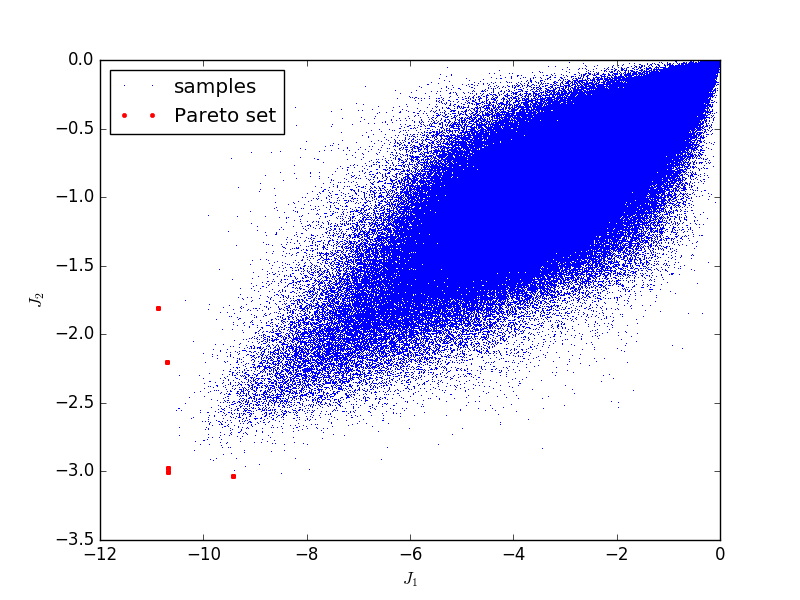
\includegraphics[width=0.8\linewidth]{pareto_12.png}
  \caption{Samples ($N=10^7$) uniformly drawn from the feasible set $\Psi$ shown
    in the cost functions space. The non-dominated samples are shown
    as bigger points.}
  \label{fig:pareto}
\end{figure}

The shadow minimum is defined by the optimization of the individual
cost functions, that is,
\begin{equation}
  J_1^* = \min_{\bar{\psi}} J_1(\bar{\psi}) \qquad
  J_2^* = \min_{\bar{\psi}} J_2(\bar{\psi})
\end{equation}
After running differential evolution over~100 runs, we obtained the
minimum values $J_1^*=-11.40$ and $J_2^*=-3.176$ (with a total variation
below~$10^{-3}$).

% The shadow minimum is defined by the optimization of the individual
% cost functions, that is,
% \begin{equation}
%   \bar{\psi_1^*} = \argmin_{\bar{\psi}} J_1(\bar{\psi}) \qquad
%   \bar{\psi_2^*} = \argmin_{\bar{\psi}} J_2(\bar{\psi})
% \end{equation}
% These minimizers corresponds to two points in the costs function
% space, say $(J_1^*,J_2^+)=( J_1(\bar{\psi_1^*}),J_2(\bar{\psi_1^*}))$
% and $(J_1^+,J_2^*)=( J_1(\bar{\psi_2^*}),J_2(\bar{\psi_2^*}))$. The
% line between these two points is called the \emph{convex hull of
%   individual minima} (CHIM)}. If the Pareto optimal set is convex,
% which from Figure~\ref{fig:pareto} seems to be the case, then it
% certainly lies below the CHIM line~\cite{das98}. After running
% differential evolution over~100 runs, we obtained the mean values
% $(J_1^*,J_2^+)=(-11.40, -2.606)$ and
% $(J_1^+,J_2^*)=(-9.260 , -3.176)$.

We applied the linear scalarization~\eqref{eq:linscal} and used a
differential evolution\footnote{We used the implementation found in
  the \emph{optimize} package of SciPy. We used the default parameters
  except for a population size of 512 and a mutation dithering range
  of~$[0.2; 0.6]$.} algorithm~\cite{storn97} on this cost function,
while ranging $\lambda$ over an equally spaced grid from 0 to 1
totalling 20 runs. Figure~\ref{fig:pm12} shows the obtained
results. The bottom left solution in the \ref{fig:pm12}(b) plot, which
approximately dominates all of the others, includes 12 of these 20
runs. 

 \begin{figure}
  \centering
  % data from rm12dep_2.npy
  \subfloat[]{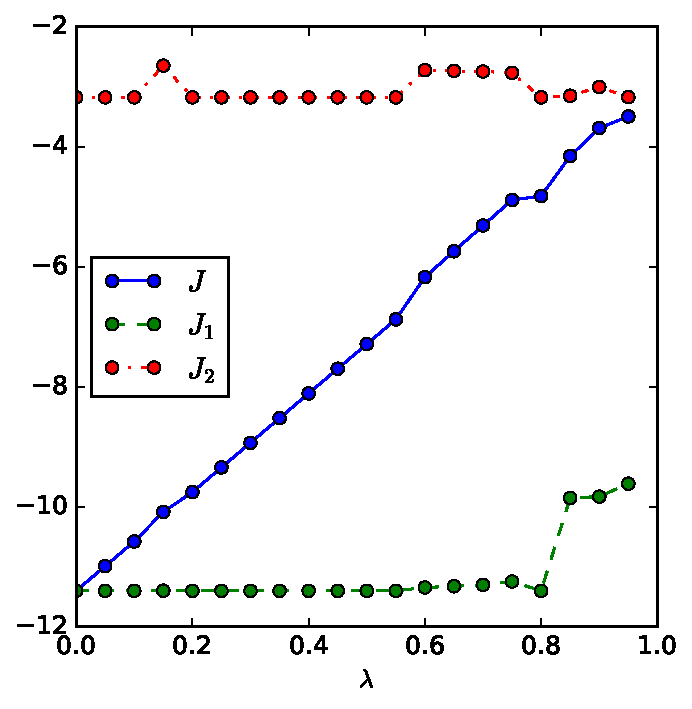
\includegraphics[width=0.33\linewidth]{out_pm12_cost.pdf}}
  \subfloat[]{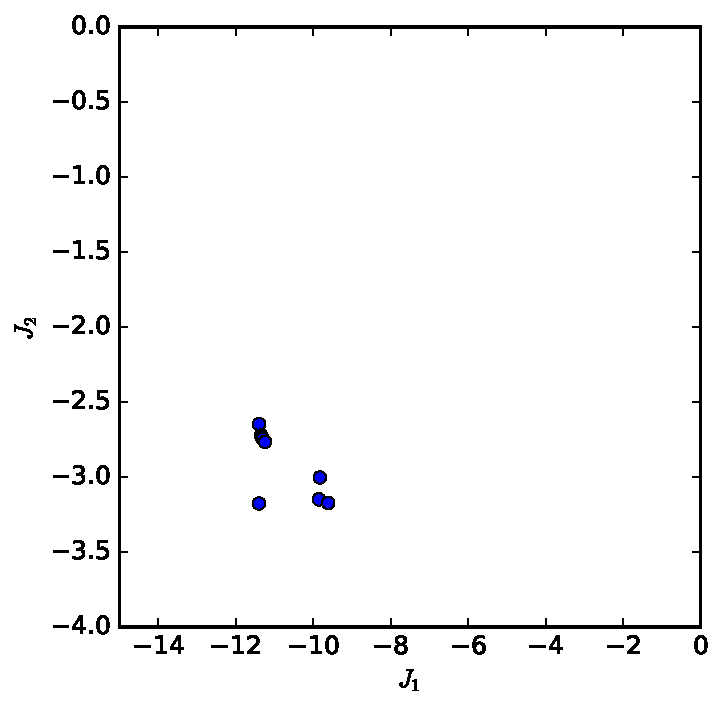
\includegraphics[width=0.33\linewidth]{out_pm12_pareto.pdf}}
  \subfloat[]{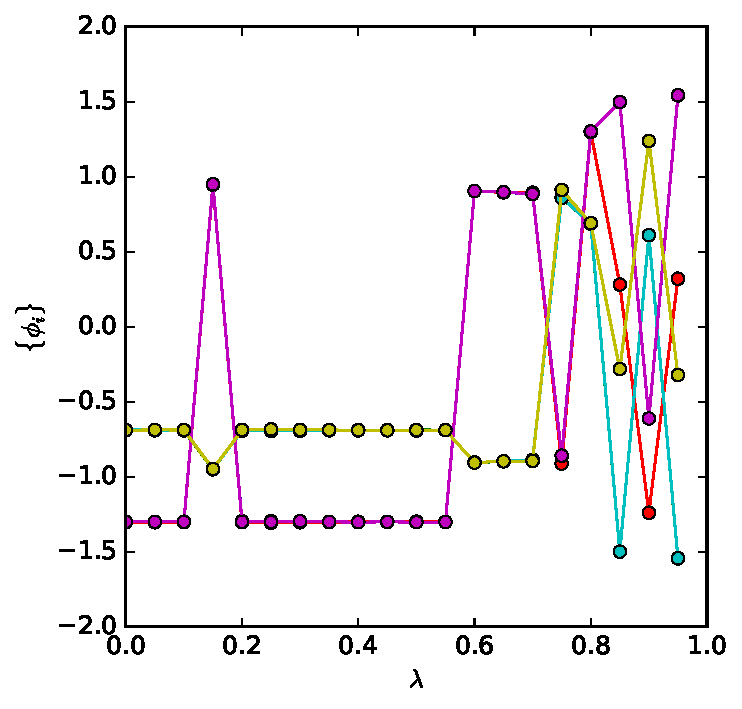
\includegraphics[width=0.33\linewidth]{out_pm12_solution.pdf}}
  \caption{Optimization results,
    from left to right: (a)~plot of $J$, $J_1=-F^\mathrm{max}$, and
    $J_2=M^\mathrm{max}$ in function of $\lambda$, (b)~solutions found
    shown in the $J_1$ and $J_2$ space, and (c)~optimized $\{\phi_i\}$
    in function of~$\lambda$.}
  \label{fig:pm12}
\end{figure}

We then ran differential evolution 100 times with
$\lambda=0.4$, an heuristically chosen within a range of $\lambda$
values where the resulting costs seem stable. From these runs, the
dominant solution, found in 24 of these 100 runs, is shown in
Table~\ref{tab:best}. Its costs are $J_1=-11.40$ and $J_2=-3.176$,
which coincide with the individual minima $J_1^*$ and $J_2^*$ found
above. That is, no other solution found has lower cost in either of
the cost functions. 

\begin{table}
  \centering
  \begin{tabular}{ccccccc}
    propeller ($i$) & 1 & 2 & 3 & 4 & 5 & 6 \\
    \hline
    $\theta_i$ & 0\textdegree & 60\textdegree & 120\textdegree & 180\textdegree & 240\textdegree & 300\textdegree \\
    $\phi_i$ & -74.54\textdegree & -39.54\textdegree & -74.57\textdegree & -39.48\textdegree & -74.49 \textdegree & -39.46 \\
    $w_i$ & -1 & 1 & -1 & 1 & -1 & 1 \\
    \hline
  \end{tabular}
  \caption{The solution found over 100 runs of the optimizer with
    $\lambda=0.4$.}
  \label{tab:best}
\end{table}

To wrap up these results, Figure~\ref{fig:costs} shows the solutions
found by differential evolution as boxplots, in three different
scenarios: the solutions for the two shadow minima
$\bar{\psi}_1^*=\arg\min J_1(\bar{\psi})$ and
$\bar{\psi}_2^*=\arg\min J_2(\bar{\psi})$, and the solutions
$\bar{\psi}_\lambda^*=\arg\min J(\bar{\psi}; \lambda)$ for
$\lambda=0.4$. Note that the minimum costs of the
$\bar{\psi}_\lambda^*$ solutions coincide with the individual
minima of $J_1^*=J_1(\bar{\psi}_1^*)$ and $J_2^*=J_2(\bar{\psi}_2^*)$.

\begin{figure}
  \centering
  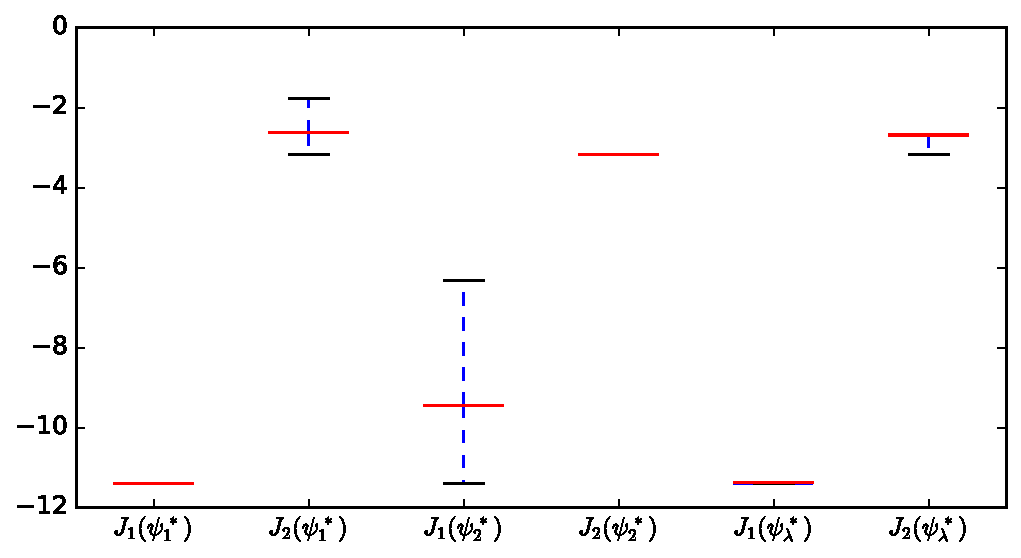
\includegraphics[width=0.8\linewidth]{out_osom12.pdf}
  \caption{Boxplots of the $J_1$ and $J_2$ costs found while
    separately minimizing, $J_1(\bar{\psi})$ (first and second
    boxplot), $J_2(\bar{\psi})$ (third and fourth boxplot), and
    $J(\bar{\psi}; \lambda)$ for $\lambda=0.4$ (fifth and
    sixth). Each boxplots represents the minimum, maximum, and median
    values.}
  \label{fig:costs}
\end{figure}

The solution in Table~\ref{tab:best} implies three of the propellers to be
almost horizontal, hindering the air flow to produce the desired
thrust. Therefore, we decided on a different solution, with the angle
values rounded from an handpicked solution from the Pareto optimal set
obtained above. Its parameters are shown in Table~\ref{tab:selected}
and its costs are $J_1=-F^\mathrm{max}=-11.40$ and
$J_2=-M^\mathrm{max}=-2.623$, that is, the same maximum force but with
82\% of the maximum torque. We preferred this solution
because the propeller angles are not as horizontal, resulting in a
significantly better air flow.
% Running the
% optimization algorithm on a restricted feasibility space parametrized
% by~$\phi$ defined as
% \begin{equation}
%   \bar{\psi} = \left(-\phi, \phi, -\phi, \phi, -\phi, \phi, -1, -1, 1, 1,
%     1, -1\right)^T
% \end{equation}
% with $\lambda=0.4$ resulted 

\begin{table}
  \centering
  \begin{tabular}{ccccccc}
    propeller ($i$) & 1 & 2 & 3 & 4 & 5 & 6 \\
    \hline
    $\theta_i$ & 0\textdegree & 60\textdegree & 120\textdegree & 180\textdegree & 240\textdegree & 300\textdegree \\
    $\phi_i$ & -55\textdegree & 55\textdegree & -55\textdegree & 55\textdegree & -55\textdegree & 55\textdegree \\
    $w_i$ & -1 & -1 & 1 & 1 & 1 & -1 \\
    \hline
  \end{tabular}
  \caption{Design parameters of the selected solution.}
  \label{tab:selected}
\end{table}


% Figure~\ref{fig:forces} shows the maximum forces and torques in set
% $\mathcal{P}_1$. The cost functions~\eqref{eq:fmax}
% and~\eqref{eq:mmax} correspond to the symmetric of the pointwise
% minimum over the three lines for each one of these plots. The
% non-convexity of the cost functions is clearly visible in this plot. When
% $\phi=0$ the maximum force is zero, since in this configuration all
% thrust is directed along the $Z$ axis: this corresponds to the
% usual configuration of hexacopters (and quadrotors, although with less
% propellers). As $|\phi|$ increases, the maximum force along directions
% other than $Z$ increases.

% \begin{figure}
%   \centering
%   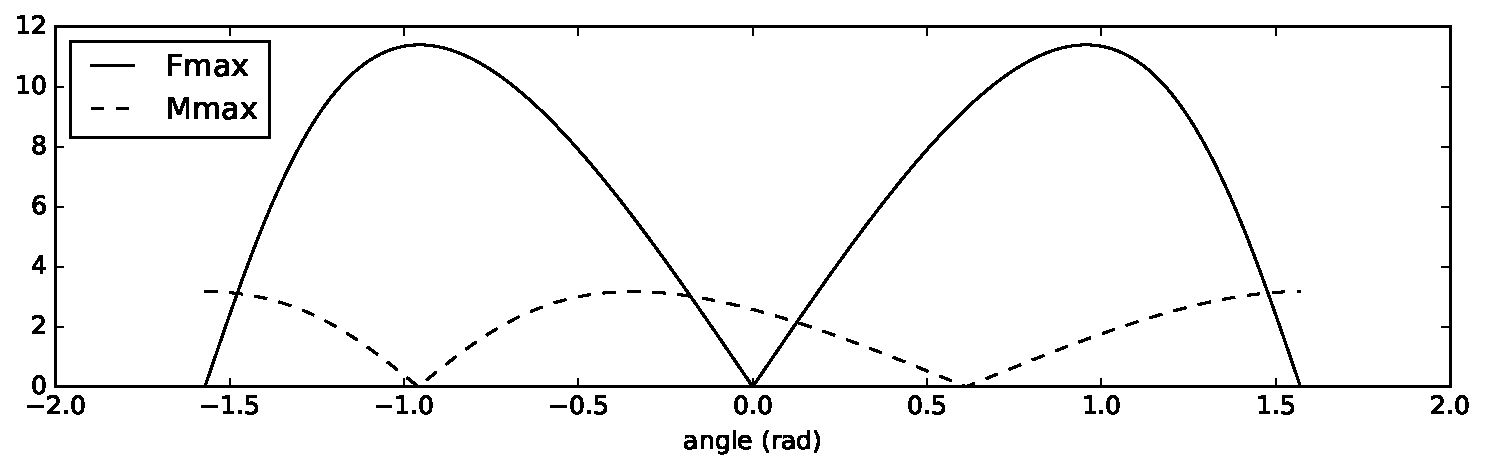
\includegraphics[width=\linewidth]{out_plot_forces.pdf}
%   \caption{Maximum force and torque, $F^\mathrm{max}$ and
%     $M^\mathrm{max}$, for each one of
%     the body frame axes while ranging across the design space
%     $\mathcal{P}_1$.}
%   \label{fig:forces}
% \end{figure}


% \begin{figure}
%   \centering
%   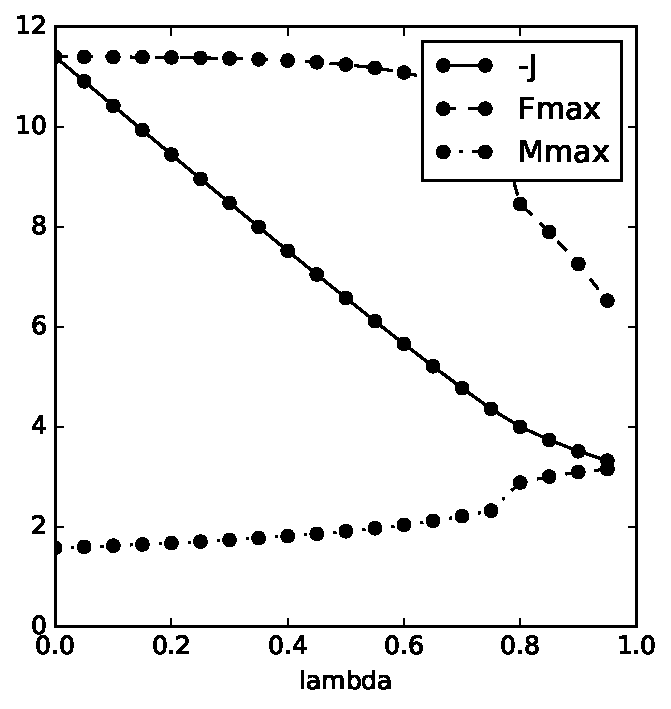
\includegraphics[width=0.32\linewidth]{out_pm1_cost.pdf} \hfill
%   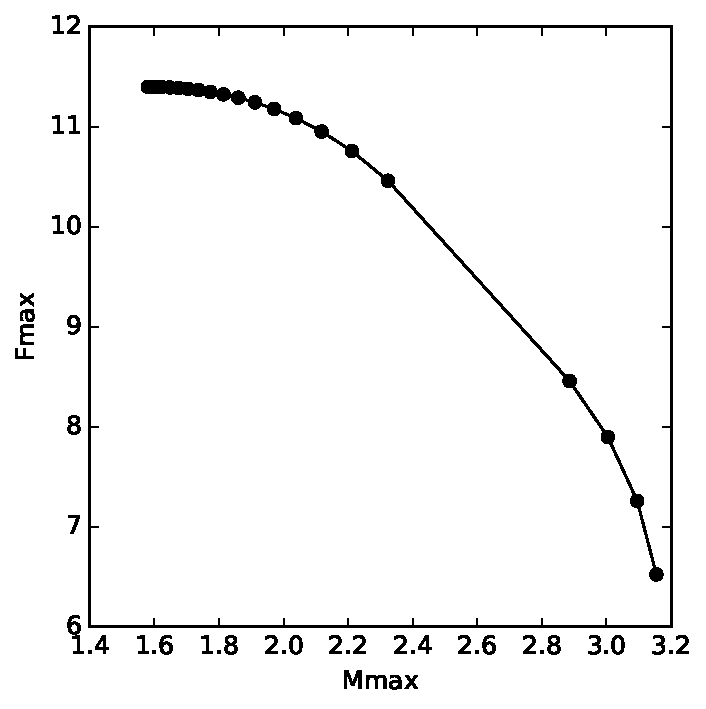
\includegraphics[width=0.32\linewidth]{out_pm1_curve.pdf} \hfill
%   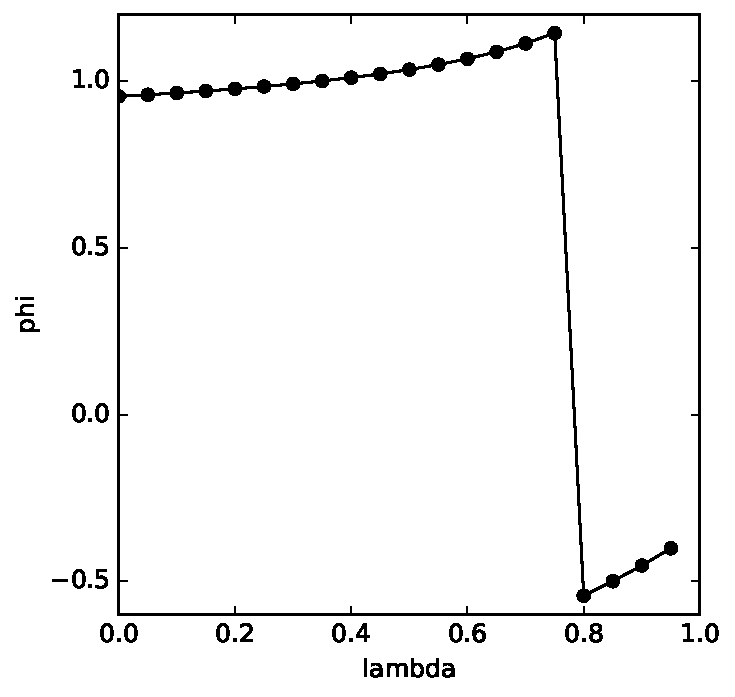
\includegraphics[width=0.32\linewidth]{out_pm1_solution.pdf} 
%   \caption{Optimization results for feasibility set $\mathcal{P}_1$,
%     from left to right: (a)~plot of $-J$, $F^\mathrm{max}$, and
%     $M^\mathrm{max}$ in function of $\lambda$, (b)~relationship between $F^\mathrm{max}$ and
%     $M^\mathrm{max}$, and (c)~optimized $\phi$ in function of $\lambda$.}
%   \label{fig:pm1}
% \end{figure}

% \begin{figure}
%   \centering
%   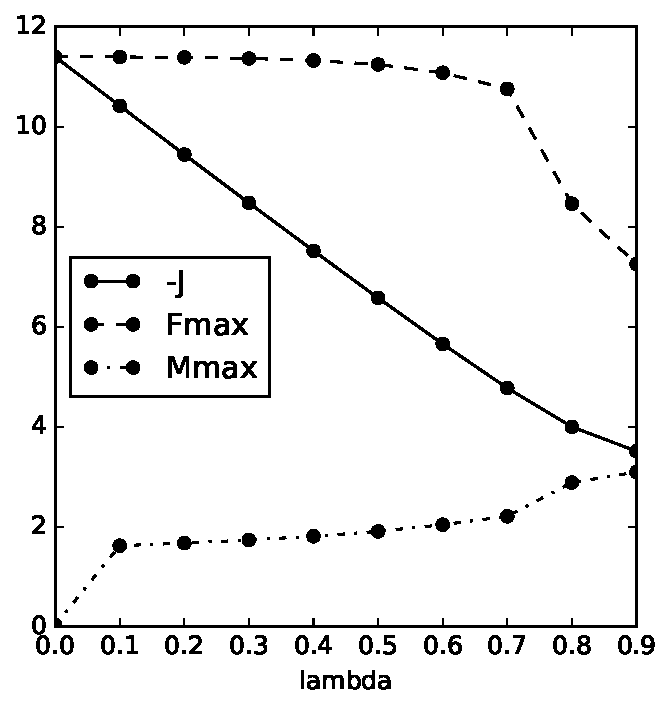
\includegraphics[width=0.32\linewidth]{out_pm3_cost.pdf} \hfill
%   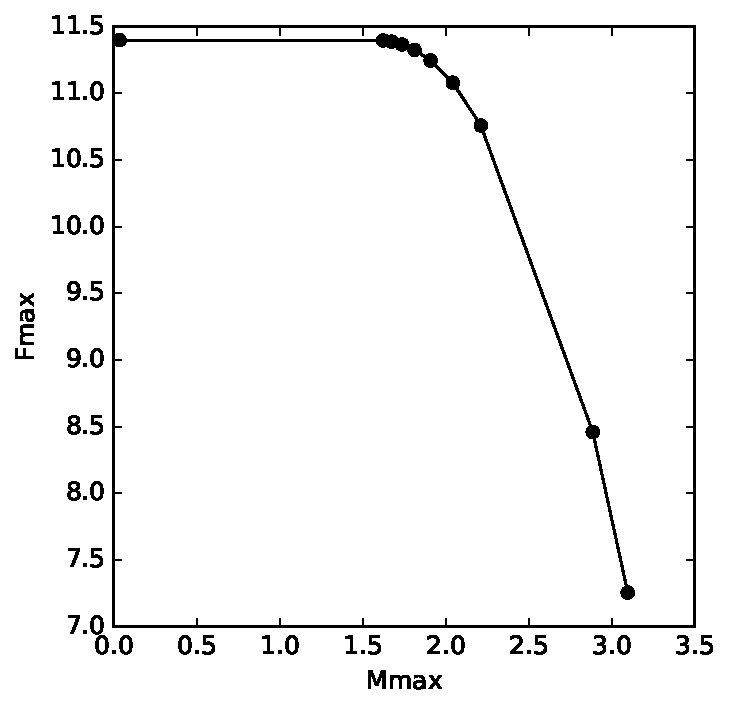
\includegraphics[width=0.32\linewidth]{out_pm3_curve.pdf} \hfill
%   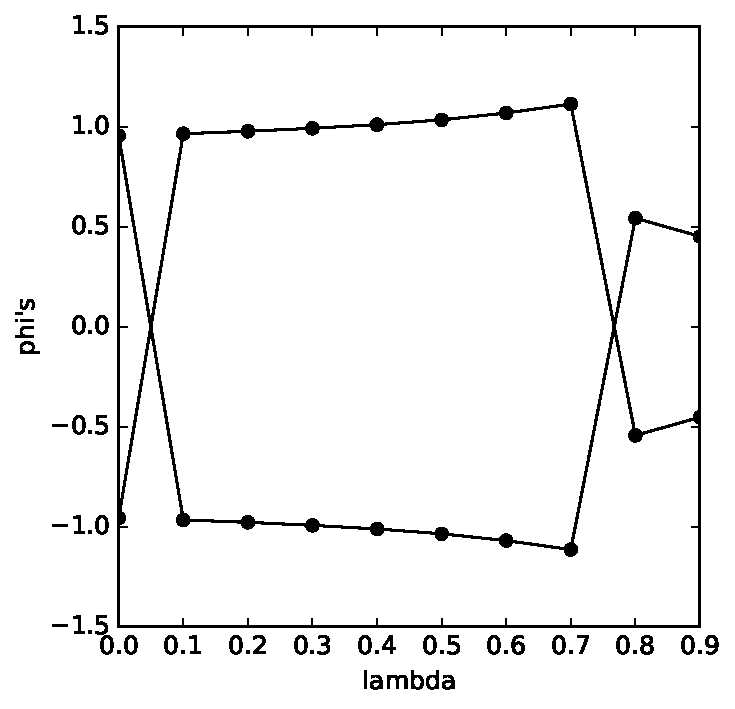
\includegraphics[width=0.32\linewidth]{out_pm3_solution.pdf} 
%   \caption{Optimization results for feasibility set $\mathcal{P}_3$,
%     same description as in Figure~\ref{fig:pm1}}
%   \label{fig:pm3}
% \end{figure}

%%% Local Variables:
%%% mode: latex
%%% TeX-master: "main"
%%% End:


\section{Position and attitude control}
\label{sec:posit-attit-contr}

The approach used for the motion control of the vehicle exploits its
holonomic design by
decoupling the translational and rotational modes. To do so, we first
apply feedback linearisation~\cite{sastry99} to the translational part
of~\eqref{eq:dynsys}:
\begin{equation}
  \label{eq:fctrl}
    \left\{
    \begin{split}
      \dot{\bar{x}} &= \bar{v} \\
      \dot{\bar{v}} &= \bar{p} \\
      \bar{F} &= m \mathbf{R}^T \bar{p}
    \end{split}
  \right.
\end{equation}
and then design a feedback controller for $\bar{p}$. Since this
dynamical system is second order, a PD controller is enough to ensure
convergence:
\begin{equation}
  \label{eq:pctrl}
  \begin{split}
    \bar{p} &= -k_x \bar{e}_x -k_v \bar{e}_v \\
    \bar{e}_x &= \bar{x} - \bar{x}_d \\
    \bar{e}_v &= \bar{v} - \bar{v}_d \\
  \end{split}
\end{equation}
where $\bar{x}_d$ and $\bar{v}_d$ are the desired position and
velocity vectors in the inertial frame~$\mathcal{I}$, and $k_x$ and
$k_v$ are the proportional and derivative gains of the PD controller.

For the attitude control we follow the convergent $SO(3)$ controller
proposed in~\cite{lee10} for the attitude of a quadrotor, negleting
the Coriolis and the angular velocity reference in the expression for
the torque, as suggested in~\cite{mahony12}:
\begin{equation}
  \label{eq:mctrl}
  \begin{split}
    \bar{M} &= -k_R\,\bar{e}_R - k_\omega\,\bar{e}_\omega \\
    \bar{e}_R &= \frac{1}{2} S^{-1}( \mathbf{R}^T_d \mathbf{R} -
    \mathbf{R}^T \mathbf{R}_d ) \\
    \bar{e}_\omega &= \omega - \mathbf{R}^T \mathbf{R}_d\,\omega_d
  \end{split}
\end{equation}
where $\mathbf{R}_d$ is the rotation matrix of the desired attitude,
$\omega_d$ is the desired angular velocity vector, with $k_R$ and
$k_\omega$ as controller gains. The $S^{-1}$ function performs the inverse
operation as the one defined in~\eqref{eq:S}, that is, recovers
the vector from a given skew-symmetric matrix.


%%% Local Variables:
%%% mode: latex
%%% TeX-master: "main"
%%% End:


\section{Preliminary validation in simulation}
\label{sec:prel-valid}

In order to provide preliminar validation of the proposed design, we simulated a simplified model of our robot with V-REP simulation framework~\cite{vrep13}. Here, we kept the size of vehicle: all motors are displaced on a 160mm radius circle, 60 degrees apart from each other, and tilted 55 degrees away from their vertical axis (see Table~\ref{tab:selected}), but with different mass and inertia, as we do not know yet have a detail design of the mass distribution. In V-REP we simulated the force and torque produced by each propeller as modeled in~\eqref{eq:Fi} and~\eqref{eq:Mi}. Thus, this simulation aims at the validation of both the design discussed in Section~\ref{sec:design-parameters} and the controller proposed in Section~\ref{sec:posit-attit-contr}.

This validation was divided into two steps: on the first, each motion mode (translation and attitude) is simulated, first, the position controller, having it move 1 meter on each direction, and then the attitude controller, by moving 70 degrees on each of its axis; on the second, we simulated a path defined by a sequence of waypoints with attitude setpoints, thus combining both controllers.

\subsection{Individual motion mode}

% The analysis of each mode enables a better adjustment of the gains of the controller and validates each controller, and component, individually. 
For this validation, the robot is holding on position $\mathbf{P_h} = (0,0,1)$, while the reference is set at $\mathbf{P_r} = (1,1,2)$. The total movement of the robot is 1 meter on each direction. On Figure~\ref{fig:position_errors} we provide the obtained results for position convergence with the proposed controller in~\eqref{eq:fctrl} and~\eqref{eq:pctrl}.

\begin{figure}
  \centering
  \subfloat[]{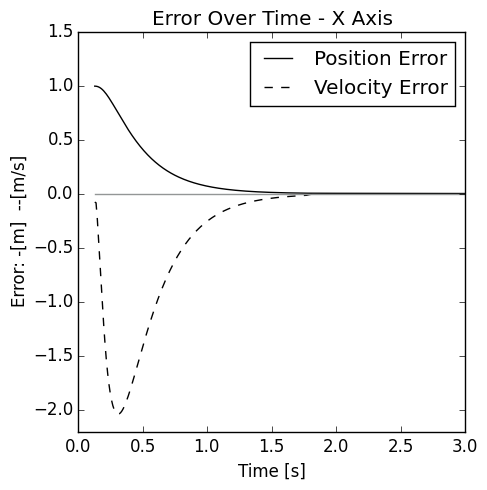
\includegraphics[width=0.33\linewidth]{px-error.png}}
  \subfloat[]{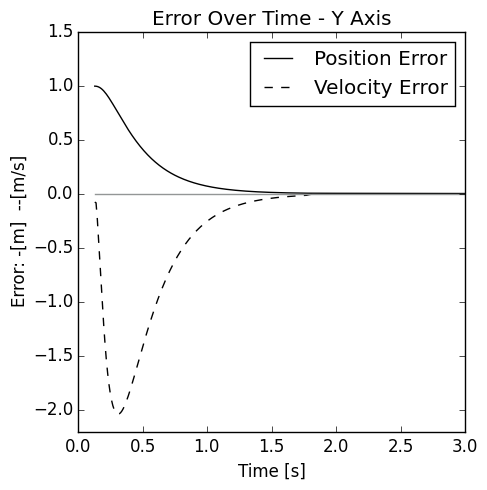
\includegraphics[width=0.33\linewidth]{py-error.png}}
  \subfloat[]{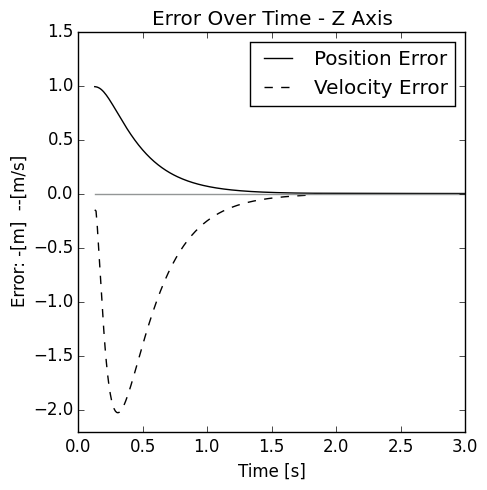
\includegraphics[width=0.33\linewidth]{pz-error.png}}
  \caption{Position Controller Error Convergence: (a)~plot of error on X component, (b)~plot of error on Y component, and (c)~plot of error on Z component.}
  \label{fig:position_errors}
\end{figure}

The three error plots are approximately equal due to the chosen gains, which are equal on all axis for this experiment: the force applied on each component is only dependent on the mass of the vehicle and position error, and not o the moment of inertia.

For the attitude controller different gains are set according to the moment of inertia of the vehicle, which resulted in a faster response for the X axis then for the Z or Y axis. The attitude of the vehicle starts as $\mathbf{R_h} = (0,0,0)$ and the reference is set as $\mathbf{R_r} = {(70\degree,0,0), (0,70\degree,0), (0,0,70\degree)}$, for rotations along X, Y and Z, respectively. The results are shown in Figure~\ref{fig:attitude_errors}.

\begin{figure}
  \centering
  \subfloat[]{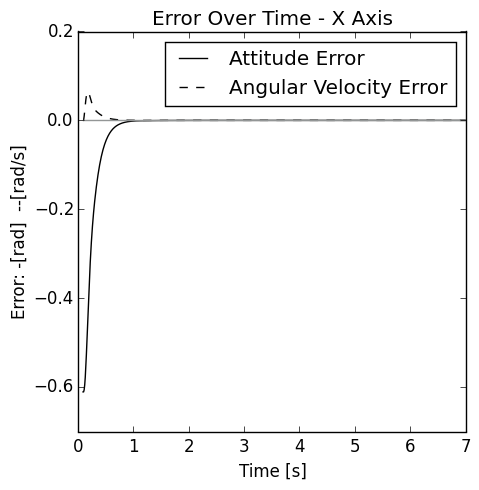
\includegraphics[width=0.33\linewidth]{rx-error.png}}
  \subfloat[]{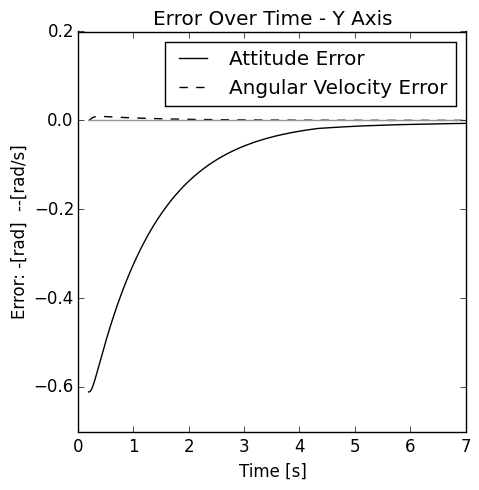
\includegraphics[width=0.33\linewidth]{ry-error.png}}
  \subfloat[]{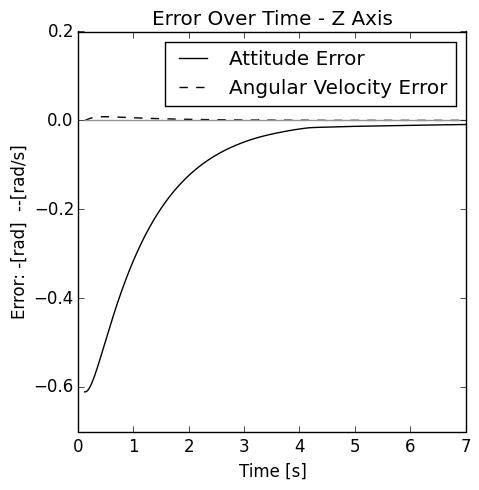
\includegraphics[width=0.33\linewidth]{rz-error.png}}
  \caption{Attitude Controller Error Convergence: (a)~plot of error on X component, (b)~plot of error on Y component, and (c)~plot of error on Z component.}
  \label{fig:attitude_errors}
\end{figure}

\subsection{Waypoint navigation}

To validate the joint position and attitude control, we used waypoint navigation: we created a virtual path composed by 6 setpoints, varying on both position and attitude. The trajectory followed by the vehicle is represented on \ref{fig:trajectory}. Plotted are both the X and Y axes of the body frame~$\mathcal{B}$ to represent its attitude. We retrieved the errors across the whole trajectory following, for both position and velocity, as well as attitude and angular velocity. These are shown in Figure~\ref{fig:nav_errors}. A video showing this simulation is available online here:~\texttt{https://youtu.be/BW1Q3lryb9c}


\begin{figure}
  \centering
  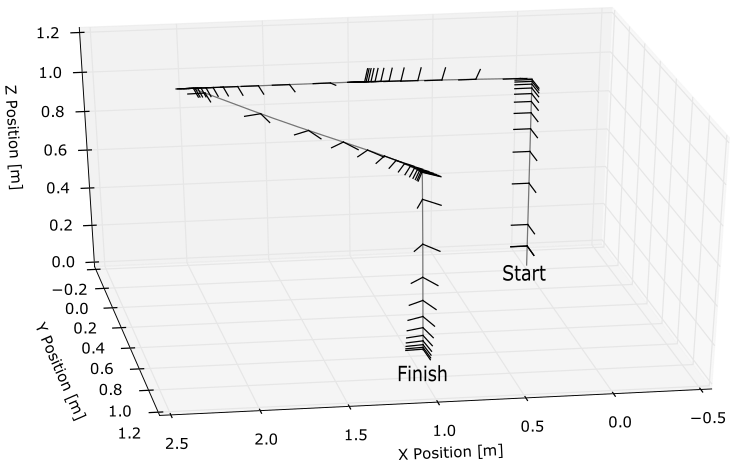
\includegraphics[width=0.8\linewidth]{3d-trajectory-names.png}
  \caption{Trajectory followed by the robot. Plotted are X and Y axis of the inertia frame~$\mathcal{I}$.}
  \label{fig:trajectory}
\end{figure}


\begin{figure}
  \centering
  \subfloat[]{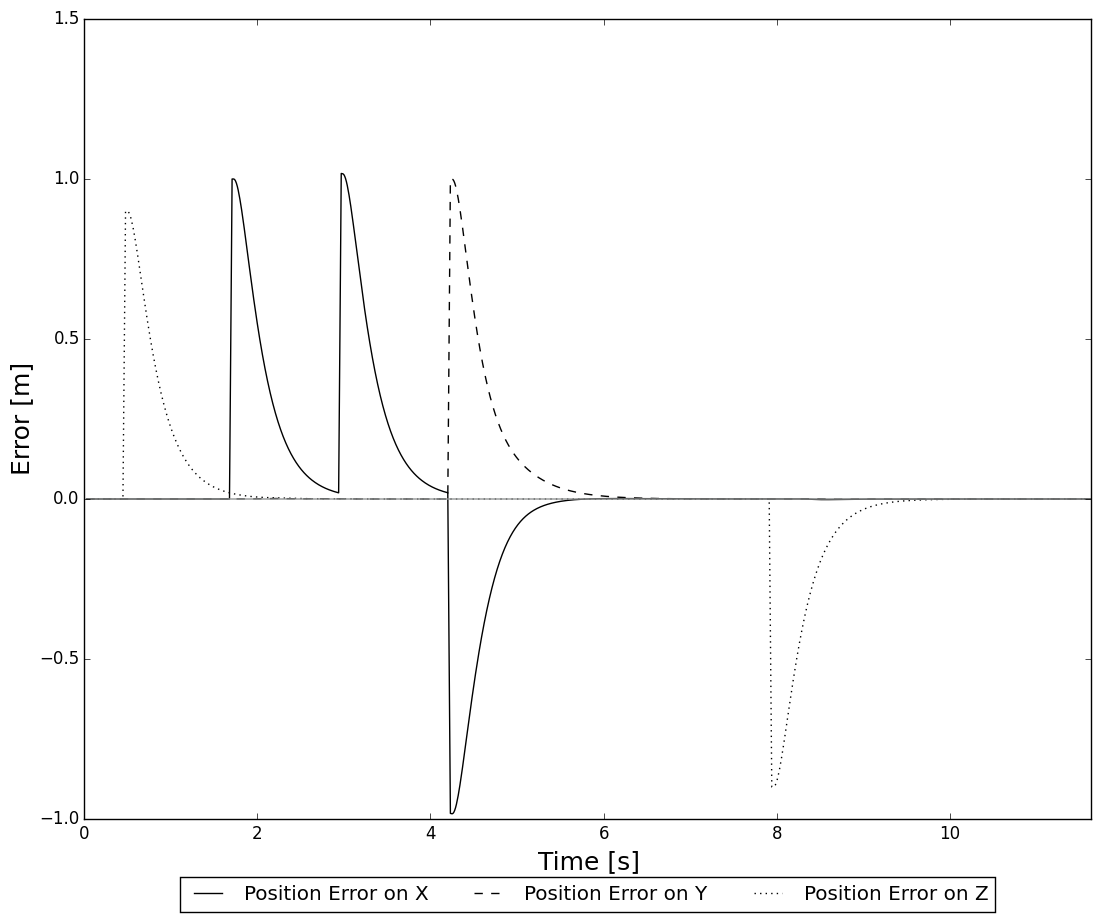
\includegraphics[width=0.45\linewidth]{traj-p-error.png}} \hfill
  \subfloat[]{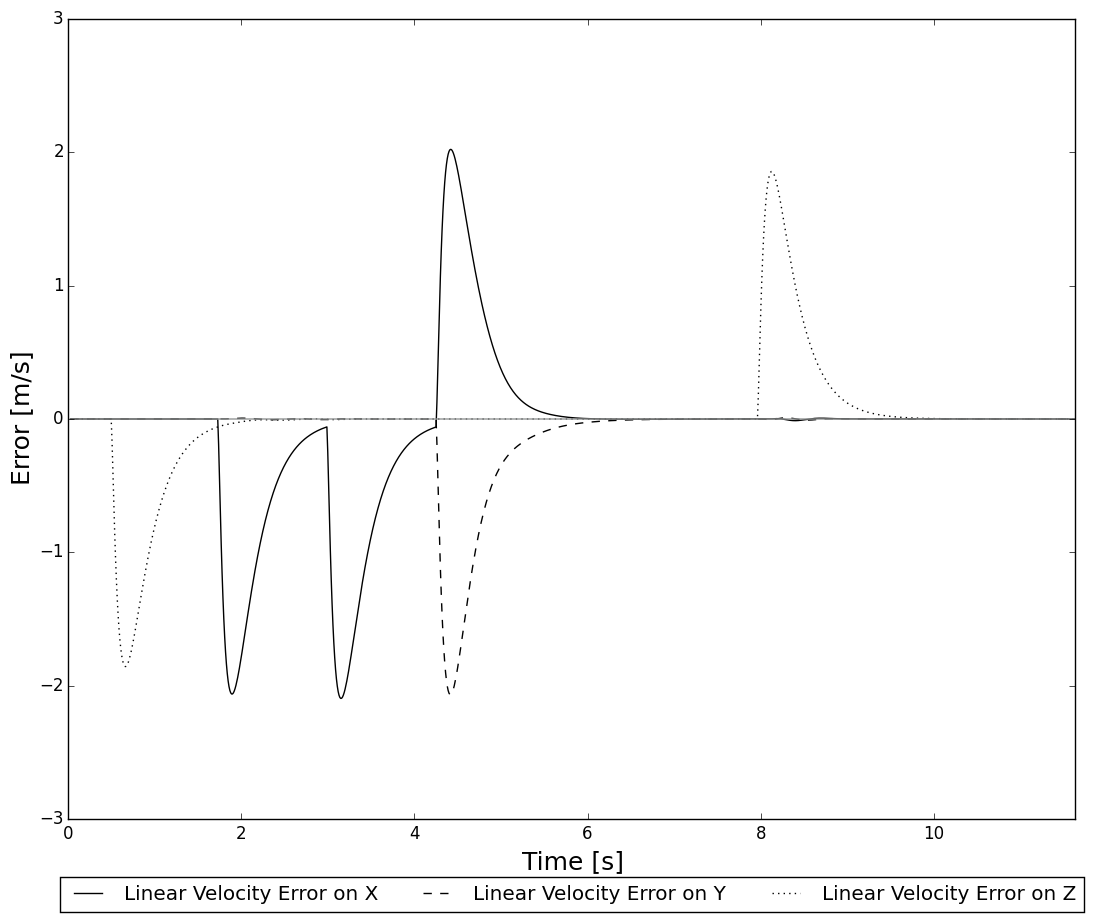
\includegraphics[width=0.45\linewidth]{traj-v-error.png}} \\
  \subfloat[]{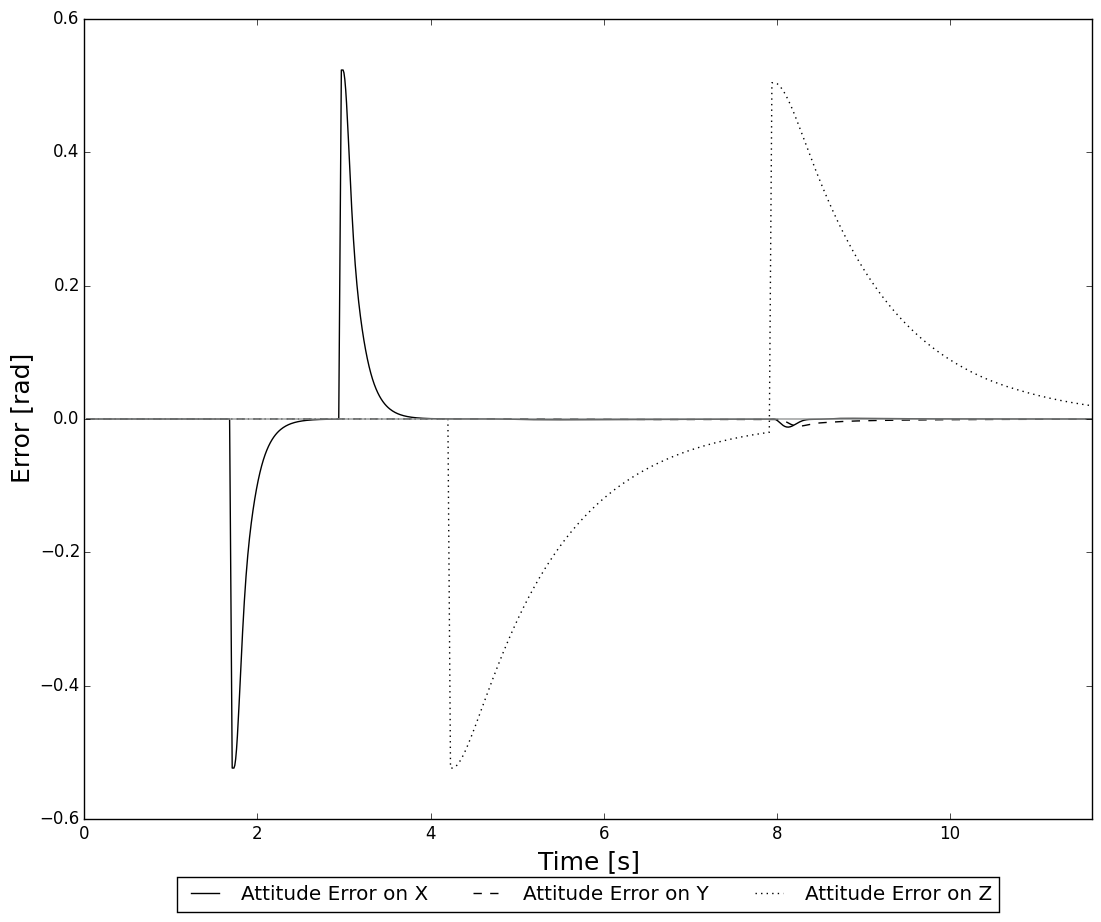
\includegraphics[width=0.45\linewidth]{traj-r-error.png}} \hfill
  \subfloat[]{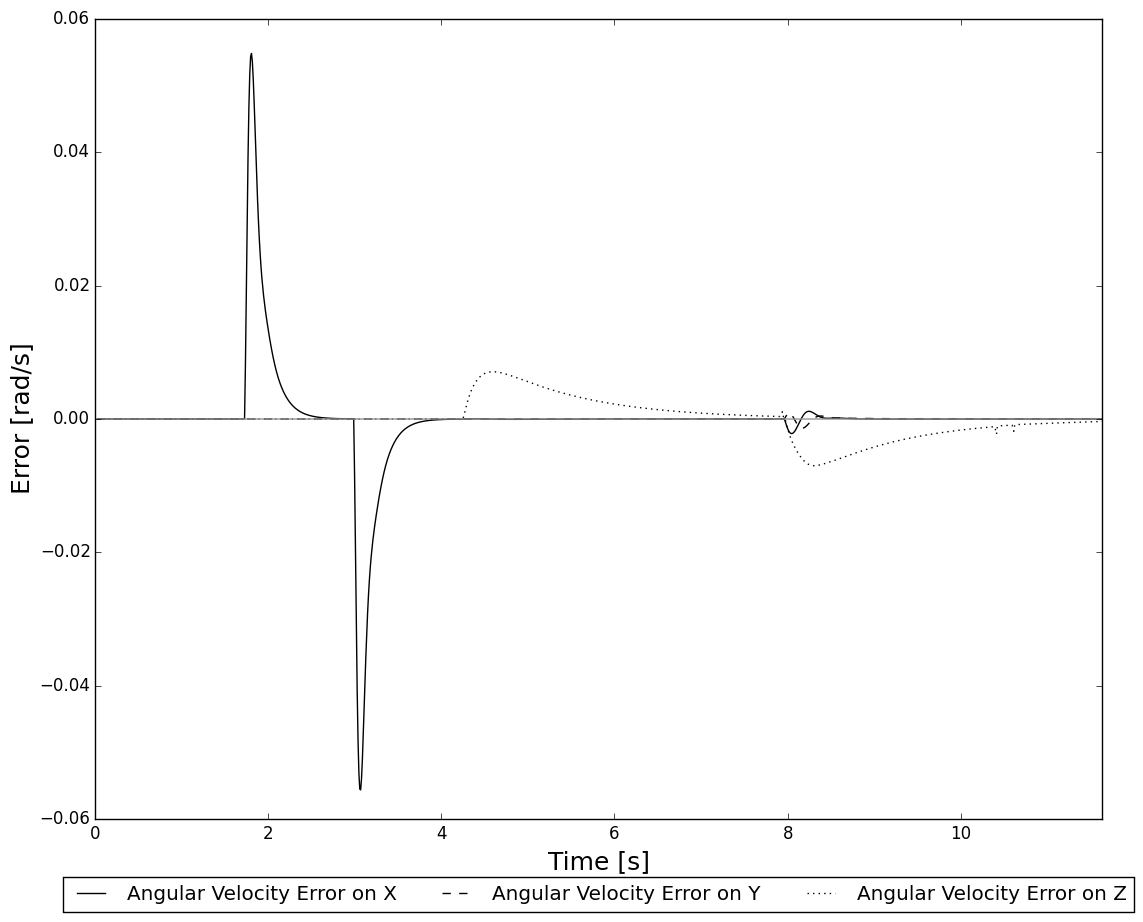
\includegraphics[width=0.45\linewidth]{traj-om-error.png}}
  \caption{Waypoint navigation position and attitude errors: (a)~error on position, (b)~error on linear velocity, (a)~error on rotation, and (b)~error on angular velocity.}
  \label{fig:nav_errors}
\end{figure}

%%% Local Variables:
%%% mode: latex
%%% TeX-master: "main"
%%% End:


\section{Conclusions and future work}
\label{sec:concl-future-work}

This paper presented a concept design of a microgravity holonomic hexarotor. We contribute with a design targeting space stations environments, aiming at collaborative work between the a fleet of these robots and humans. In addition,the solution provides room for extension modules that may be used for increased functionalities and to host microgravity experimental test-beds.

We used an multi-criteria optimization approach to guide the design parameters of the proposed propulsion system. We also proposed a convergent controller for the vehicle, and validated our design in a realistic physics-based simulator. Simulation results show the vehicle navigating between waypoints.

In the future, some work should be done to enhance the design , namely: to study the robustness to the variation of the design parameters around the proposed design, to analyse the controller's robustness to structural and sensor perturbations, and lastly, to validate on the simulator the vehicle with the expected mass and moment of inertia.

%%% Local Variables:
%%% mode: latex
%%% TeX-master: "main"
%%% End:


\section*{Acknowledgments}
\label{sec:acknowledgments}

The authors are grateful to André Santos for the CAD modeling of the
vehicle and the renderings presented in this paper. This work was
supported by the FCT project~[UID/EEA/50009/2013].

\bibliography{biblio}
\bibliographystyle{plain}



\end{document}
